%!TEX TS-program = xelatex
\documentclass[10pt]{article}
\usepackage[a4paper,margin=0mm]{geometry}
\usepackage[no-math]{fontspec}
\usepackage{tikz}
\usepackage{amsmath}
\usepackage{amssymb}
\usepackage{bm}
\usepackage{graphicx}
\usepackage{xcolor}
\usepackage[protrusion=true,expansion=false]{microtype}
\usepackage{ragged2e}
\usepackage{qrcode}
\usepackage{eso-pic}
\usepackage{setspace}
\usepackage{calc}
\usepackage{array}
\usepackage{multicol}
\usepackage{hyperref}
\hypersetup{hidelinks}

\setmainfont{EBGaramond-Regular.otf}[
  Path=/usr/local/texlive/2024/texmf-dist/fonts/opentype/public/ebgaramond/,
  BoldFont=EBGaramond-Bold.otf,
  ItalicFont=EBGaramond-Italic.otf,
  BoldItalicFont=EBGaramond-BoldItalic.otf,
  Ligatures=TeX,
  RawFeature={+liga,-dlig,-hlig}]
\newfontfamily\relationfont{EBGaramond-Regular.otf}[
  Path=/usr/local/texlive/2024/texmf-dist/fonts/opentype/public/ebgaramond/,
  BoldFont=EBGaramond-Bold.otf,
  ItalicFont=EBGaramond-Italic.otf,
  BoldItalicFont=EBGaramond-BoldItalic.otf,
  Ligatures=TeX,
  RawFeature={+liga,+dlig,+hlig}]
\newfontfamily\flourishfont{Junicode-Regular.otf}[
  Path=/usr/local/texlive/2024/texmf-dist/fonts/opentype/public/junicode/,
  BoldFont=Junicode-Bold.otf,
  ItalicFont=Junicode-Italic.otf,
  BoldItalicFont=Junicode-BoldItalic.otf,
  Ligatures=TeX,
  RawFeature={+liga,+dlig,+hlig,+calt,+ss01}]
\newfontfamily\metafont{lmroman10-regular.otf}[
  Path=/usr/local/texlive/2024/texmf-dist/fonts/opentype/public/lm/,
  Scale=MatchLowercase]
\newcommand{\displayfont}{\rmfamily\bfseries}
\definecolor{paper}{HTML}{FFFFFF}
\definecolor{ink}{HTML}{000000}
\definecolor{signal}{HTML}{000000}
\pagecolor{paper}\color{ink}
\pagestyle{empty}
\setlength{\parindent}{0pt}
\newlength{\mainmeasure}
\setlength{\mainmeasure}{.66\paperwidth}
% All mathematics is isolated from the document's text faces and locked to
% classic Computer Modern Roman and its companion Computer Modern math fonts.
% Even explicit sans-serif or monospaced math requests resolve to serif CMR.
% Do not load unicode-math or redirect the OML/OMS/OT1 math families.
\SetMathAlphabet{\mathrm}{normal}{OT1}{cmr}{m}{n}
\SetMathAlphabet{\mathbf}{normal}{OT1}{cmr}{bx}{n}
\SetMathAlphabet{\mathit}{normal}{OT1}{cmr}{m}{it}
\SetMathAlphabet{\mathsf}{normal}{OT1}{cmr}{m}{n}
\SetMathAlphabet{\mathtt}{normal}{OT1}{cmr}{m}{n}
\SetMathAlphabet{\mathrm}{bold}{OT1}{cmr}{bx}{n}
\SetMathAlphabet{\mathbf}{bold}{OT1}{cmr}{bx}{n}
\SetMathAlphabet{\mathit}{bold}{OT1}{cmr}{bx}{it}
\SetMathAlphabet{\mathsf}{bold}{OT1}{cmr}{bx}{n}
\SetMathAlphabet{\mathtt}{bold}{OT1}{cmr}{bx}{n}
% Force visibly bold Computer Modern mathematics without borrowing the text font.
\newcommand{\CMboldmath}[1]{{\boldmath\ensuremath{\boldsymbol{#1}}}}

\newcommand{\meta}[2]{%
  \begin{tikzpicture}[remember picture,overlay]
    \draw[signal,line width=.55pt] ([xshift=11mm,yshift=-11mm]current page.north west) rectangle ++(44mm,-17mm);
    \node[anchor=north west,align=left,font=\metafont\fontsize{6.2}{7.2}\selectfont] at ([xshift=13mm,yshift=-13mm]current page.north west) {TAKE OVER\\FOTOGRAFISKA TALLINN\\#1};
    \node[anchor=north east,text=signal,font=\metafont\fontsize{6.2}{7.2}\selectfont] at ([xshift=53mm,yshift=-25mm]current page.north west) {#2};
  \end{tikzpicture}\par}

\newcommand{\folio}[1]{\begin{tikzpicture}[remember picture,overlay]
\node[anchor=south east,text=signal,font=\metafont\fontsize{6}{7}\selectfont] at ([xshift=-10mm,yshift=8mm]current page.south east) {#1 / 24};
\end{tikzpicture}\par}

\newcommand{\statement}[1]{{\RaggedRight\displayfont\color{signal}\fontsize{36}{34}\selectfont\MakeUppercase{#1}\par}}
\newcommand{\bigstatement}[1]{{\RaggedRight\displayfont\color{signal}\fontsize{55}{51}\selectfont\MakeUppercase{#1}\par}}
\newcommand{\smallcapsline}[1]{{\metafont\color{signal}\fontsize{7}{9}\selectfont\MakeUppercase{#1}}}
\newcommand{\sectionnumber}[1]{{\rmfamily\bfseries\color{signal}\fontsize{28}{28}\selectfont #1.}}
\newcommand{\sidelegend}{\begin{tikzpicture}[remember picture,overlay]
  \node[rotate=90,anchor=south west,text=signal,font=\rmfamily\bfseries\fontsize{7}{8}\selectfont]
  at ([xshift=10mm,yshift=12mm]current page.south west)
  {IMAGE / VOICE / PLACE / PRACTICE / RELATION / NEXT};
  \draw[signal,line width=.5pt] ([xshift=11mm,yshift=12mm]current page.south west)--([xshift=11mm,yshift=82mm]current page.south west);
\end{tikzpicture}\par}

\newcommand{\photobox}[2][.72\paperheight]{%
  \begin{tikzpicture}
    \fill[white] (0,0) rectangle (\linewidth-.8pt,#1);
    \draw[signal,line width=.7pt] (0,0) rectangle (\linewidth-.8pt,#1);
    \draw[signal,line width=.35pt] (0,0)--(\linewidth-.8pt,#1) (0,#1)--(\linewidth-.8pt,0);
    \node[fill=paper,inner sep=4mm,align=center,text=signal,font=\metafont\fontsize{8}{10}\selectfont] at (.5\linewidth-.4pt,.5#1) {PHOTOGRAPH PLACEHOLDER\\#2};
  \end{tikzpicture}}

% Three successive hand-drawn QR states. These are deliberately not scannable
% yet: each portal records a stage in the movement from sign to operative code.
\newcommand{\qrprogression}[4]{%
  \begin{tikzpicture}[x=1mm,y=1mm]
    \node[inner sep=0,fill=black] at (10,10)
      {\includegraphics[width=20mm,height=20mm,keepaspectratio]{assets/qr_progression/#1}};
    \node[inner sep=0,fill=black] at (31.5,10)
      {\includegraphics[width=20mm,height=20mm,keepaspectratio]{assets/qr_progression/#2}};
    \node[inner sep=0,fill=black] at (53,10)
      {\includegraphics[width=20mm,height=20mm,keepaspectratio]{assets/qr_progression/#3}};
    \draw[signal,line width=.45pt,->] (0,-2)--(63,-2);
    \node[anchor=north,text=signal,font=\metafont\fontsize{6.3}{7.5}\selectfont]
      at (31.5,-3) {#4};
  \end{tikzpicture}}

\newcommand{\masonrywidth}[5]{%
  \begin{scope}
    \clip (#2,#3) rectangle ++(#4,-#5);
    \node[anchor=center,inner sep=0] at ({#2+#4/2},{#3-#5/2})
      {\includegraphics[width=#4mm]{#1}};
  \end{scope}}
\newcommand{\masonryheight}[5]{%
  \begin{scope}
    \clip (#2,#3) rectangle ++(#4,-#5);
    \node[anchor=center,inner sep=0] at ({#2+#4/2},{#3-#5/2})
      {\includegraphics[height=#5mm]{#1}};
  \end{scope}}
\newcommand{\missingmasonry}[4]{%
  \draw[signal,line width=.55pt] (#1,#2) rectangle ++(#3,-#4);
  \draw[signal,line width=.7pt] (#1,#2)--++(#3,-#4)
    (#1,{#2-#4})--++(#3,#4);
  \node[fill=paper,inner sep=1.2mm,font=\metafont\fontsize{6.2}{7}\selectfont]
    at ({#1+#3/2},{#2-#4/2}) {YET MISSING};}
\newcommand{\galleryfit}[6]{%
  \draw[signal,line width=.45pt] (#2,#3) rectangle ++(#4,-#5);
  \node[anchor=center,inner sep=0] at ({#2+#4/2},{#3-#5/2})
    {\includegraphics[width=\dimexpr#4mm-2mm\relax,height=\dimexpr#5mm-2mm\relax,keepaspectratio]{#1}};
  \node[anchor=north west,fill=white,inner sep=1mm,font=\metafont\fontsize{5.8}{6.5}\selectfont]
    at ({#2+1},{#3-1}) {#6};}
\newcommand{\gallerymissing}[5]{%
  \draw[signal,line width=.55pt] (#1,#2) rectangle ++(#3,-#4);
  \draw[signal,line width=.55pt] (#1,#2)--++(#3,-#4) (#1,{#2-#4})--++(#3,#4);
  \node[fill=white,inner sep=1mm,font=\metafont\fontsize{5.8}{6.5}\selectfont]
    at ({#1+#3/2},{#2-#4/2}) {#5 / UNALLOCATED};}

\newcommand{\networkbg}[1]{%
\begin{tikzpicture}[remember picture,overlay]
\foreach \x/\y in {20/25,44/18,72/28,88/46,67/67,38/72,16/58}{\fill[black] ([xshift=\x mm,yshift=\y mm]current page.south west) circle (.8pt);}
\draw[black,line width=.25pt] ([xshift=20mm,yshift=25mm]current page.south west)--([xshift=44mm,yshift=18mm]current page.south west)--([xshift=72mm,yshift=28mm]current page.south west)--([xshift=88mm,yshift=46mm]current page.south west);
\draw[black,line width=.25pt] ([xshift=44mm,yshift=18mm]current page.south west)--([xshift=67mm,yshift=67mm]current page.south west)--([xshift=38mm,yshift=72mm]current page.south west)--([xshift=16mm,yshift=58mm]current page.south west);
\end{tikzpicture}\par}

\begin{document}

% 1 START
\meta{COMMUNITY GALLERY}{START}\folio{01}\sidelegend
\vspace*{55mm}
\begin{center}
  {\rmfamily\itshape\fontsize{12}{15}\selectfont (the process of)}\par
  \vspace{5mm}
  % Genuine Computer Modern mathematics, enlarged without changing family.
  {\boldmath\scalebox{4.15}{$\displaystyle \boldsymbol{+\! *\! /}$}}\par
  \vspace{7mm}
  {\metafont\fontsize{9}{12}\selectfont INTERACTIVE IN PROGRESS}\par
  \vspace{16mm}
  \qrprogression{inv_qr_01_450d.png}{inv_qr_02_4902.png}{inv_qr_03_6fb1.png}%
    {01--03 / ABSTRACT SIGNAL}
\end{center}
\vfill
\hspace*{14mm}\smallcapsline{This application is the first event in the process.}\vspace{15mm}
\newpage

% 2 CHIME
\meta{INITIAL CONDITION}{CHIME}\folio{02}\sidelegend
\begin{tikzpicture}[remember picture,overlay]
  \node[anchor=north west,align=left,text width=38mm,font=\fontsize{8.8}{11.2}\selectfont]
  at ([xshift=14mm,yshift=168mm]current page.south west) {%
    \textbf{TAKE OVER is an initial condition looking for consequences.}\\[5mm]
    \textbf{WHAT IS THIS NOT?}\\[3mm]
    Everything asks to be continued.\\
    Enter anywhere.\\
    Change what follows.};
\end{tikzpicture}\par
\vspace*{46mm}\hspace*{62mm}
\begin{minipage}{\mainmeasure}
  \bigstatement{TAKE\\OVER.}
  \vspace{8mm}
  {\fontsize{17}{22}\selectfont through the \textbf{WALL}.}\par
  \vspace{18mm}
  {\fontsize{18}{24}\selectfont
    image $\rightarrow$ voice $\rightarrow$ sound\\
    $\rightarrow$ person $\rightarrow$ practice\\
    $\rightarrow$ relation $\rightarrow$ next}
  \par\vspace{18mm}
  {\fontsize{13}{17}\selectfont\itshape an initial condition.}\par
\end{minipage}
\newpage

% 3 ABSTRACT
\meta{APPLICATION}{INITIAL CONDITION}\folio{03}\sidelegend
\vspace*{45mm}\hspace*{62mm}
\begin{minipage}{\mainmeasure}
  \sectionnumber{0}\par\vspace{1mm}
  {\displayfont\color{signal}\fontsize{24}{24}\selectfont INITIAL CONDITION.}\par\vspace{8mm}
  {\fontsize{12.5}{16}\selectfont
    A photographic sequence of abandoned churches, damaged architectures, bodies, apertures, and objects whose meaning changes as they carry on, frame to frame.\\[5mm]
    Beside and within the photographic work, encoded portals open another layer: voices, field recordings and other sounds. The image does not explain; the sound does not close it. Each can spark another connection.\\[5mm]
    TAKE OVER begins from what remains. We inherit architectures, images, memories, relationships, sounds, and debris. It asks what can begin inside spaces opened by something else. Community is a process.
  }
\end{minipage}
\newpage

% 4 SHORT PROJECT DESCRIPTION
\meta{APPLICATION}{SHORT PROJECT DESCRIPTION}\folio{04}\sidelegend
\vspace*{39mm}\hspace*{62mm}
\begin{minipage}{\mainmeasure}
  {\RaggedRight\displayfont\fontsize{29}{28}\selectfont
    TAKE OVER\par}
  \vspace{2mm}
  {\relationfont\fontsize{12}{15}\selectfont\itshape
    interactive in progress / extinction in progress\par}
  \vspace{9mm}
  {\fontsize{10.4}{13.2}\selectfont\justifying
    There is a church. More precisely, there is what remains of one: stone,
    apertures, funerary inscriptions, broken surfaces, light, acoustic cavities.
    Before \textit{church} became the name of a building or institution,
    \textit{ekkles\'ia} named an assembly---people called together. Here the
    architecture remains. The ecclesia does not. This is our initial condition.\par\vspace{4mm}

    TAKE OVER begins from what remains and asks what can happen next. A
    photographic sequence moves through abandoned churches, bodies, openings,
    and objects whose meaning changes frame to frame. A square appears. At first
    it has no known function. Exposed, carried, displaced, and observed, it moves
    from signal to token to code to portal. The image does not explain the sound;
    the sound does not close the image; a voice does not resolve the photograph.
    Each produces another possible direction.\par\vspace{3mm}

    \[
      \mathrm{image}\rightarrow\mathrm{voice}\rightarrow\mathrm{sound}
      \rightarrow\mathrm{person}\rightarrow\mathrm{practice}
      \rightarrow\mathrm{relation}\rightarrow\mathrm{next}.
    \]

    The project approaches community as an irreversible system: not an object,
    a sum of individuals, or consensus, but an evolving configuration of
    relations. Ave Palm, Mai-Brit T\"anava, Kenn-Eerik Kannike, and Andrés A.
    Le\'on Baldelli / kumiori III remain attributable authors. Difference remains
    visible while relations grow.\par\vspace{4mm}

    The open call gives us fifteen photographic positions. We allocate twelve
    and reserve three---twenty percent of the wall---for contributions that have
    not surfaced yet:
    \[
      12+\square+\square+\square=15.
    \]
    Vacancy is not outside the work. It is an active variable. Photographs lead
    through provisional QR portals toward voices, field recordings, sound, and
    an evolving digital surface. The wall is not simply where the work is shown;
    it is another initial condition.\par\vspace{4mm}

    TAKE OVER does not restore the vanished assembly or reconstruct a previous
    order. It asks whether another assembly can emerge from the remains without
    absorbing those who enter. Someone enters. Something changes. Another
    possibility becomes admissible. The configuration changes again.}
  \vspace{7mm}
  {\displayfont\fontsize{14}{16}\selectfont
    TAKE OVER THE WALL. TAKE OVER THE OPENING. TAKE OVER THE SOUND.\par
    TAKE OVER WHAT FOLLOWS.\quad PASS IT ON.}
\end{minipage}
\newpage

% 5 RATIONALE
\meta{RATIONALE}{ENTRY 00}\folio{05}\sidelegend
\vspace*{51mm}\hspace*{62mm}
\begin{minipage}{\mainmeasure}
  \setlength{\parindent}{0pt}
  \justifying
  {\flourishfont
    {\fontsize{18}{23}\selectfont
      \hangindent=13mm\hangafter=1
      \textbf{rationale}\enspace \textit{n.}\enspace
      From what remains: architectures, images, memories, relationships, sounds,
      and debris. TAKE OVER asks what can begin inside spaces opened by something
      else. --- Community is not presented as a stable object but as a process.
      Photography opens to voice; voice opens to sound. Sound opens to another
      person; another person brings another practice. The work grows through these
      relations.\par}
    \vspace{13mm}
    {\fontsize{14}{19}\selectfont
      \textbf{Deriv.}\enspace
      \textit{image-to-voice; voice-to-sound; sound-to-person; person-to-practice;
      practice-to-relation; relation-to-next.}\par}}
  \vspace{13mm}
  {\relationfont\fontsize{16}{20}\selectfont
    \hangindent=11mm\hangafter=1
    \textbf{church}\enspace \textit{n.}\enspace
    A gathered body; also, the place in which it gathers. In TAKE OVER, the
    church is an inherited architecture of assembly, memory, vacancy, and
    return: a photographed threshold that holds what remains while making room
    for another voice, another sound, another relation.\par}
  \vspace{20mm}
  {\fontsize{12}{16}\selectfont
    An initial condition looking for consequences. Everything asks to be
    continued. Enter anywhere. Change what follows.}
\end{minipage}
\newpage

% 5 SYSTEM
\meta{SYSTEM}{PERTURBATION}\folio{06}\sidelegend
\vspace*{57mm}
\begin{center}
  {\fontsize{38}{45}\selectfont
    \[
      7+5+\cdots=12
    \]}
  \vspace{16mm}
  {\fontsize{13}{17}\selectfont\itshape initial allocation}\par
  \vspace{30mm}
  {\fontsize{38}{45}\selectfont
    \[
      12+\square+\square+\square=15
    \]}
  \vspace{16mm}
  {\fontsize{13}{17}\selectfont\itshape positions reserved for what has not surfaced yet}\par
\end{center}
\newpage

% 5 EXHIBITION
\meta{EXHIBITION}{SYSTEM OF RELATIONS}\folio{07}\sidelegend
\vspace*{43mm}\hspace*{62mm}
\begin{minipage}{\mainmeasure}
  {\RaggedRight\displayfont\fontsize{27}{28}\selectfont THE WALL IS THE\\INITIAL CONDITION.}\par
  \vspace{9mm}
  {\fontsize{11.5}{15}\selectfont
    The exhibition combines photographic works by the initial contributors with small QR portals connecting selected works to voices, sound, and the evolving digital surface. It does not attempt to fill every available position. Some positions remain unallocated: scarce exhibition space is reserved for contributions that have not surfaced yet.}
\end{minipage}\par
\vspace{12mm}
\hspace*{14mm}\begin{minipage}{182mm}
  \begin{tikzpicture}[x=1mm,y=1mm]
    \draw[signal,line width=.55pt,->] (24,73)--(68,83);
    \draw[signal,line width=.55pt,->] (68,83)--(114,73);
    \draw[signal,line width=.55pt,->] (114,73)--(156,83);
    \draw[signal,line width=.55pt,->] (156,83)--(151,41);
    \draw[signal,line width=.55pt,->] (151,41)--(98,30);
    \draw[signal,line width=.55pt,->] (98,30)--(38,39);

    \node[anchor=south west,inner sep=0,draw=signal,line width=.45pt,rotate=-2]
      at (0,58) {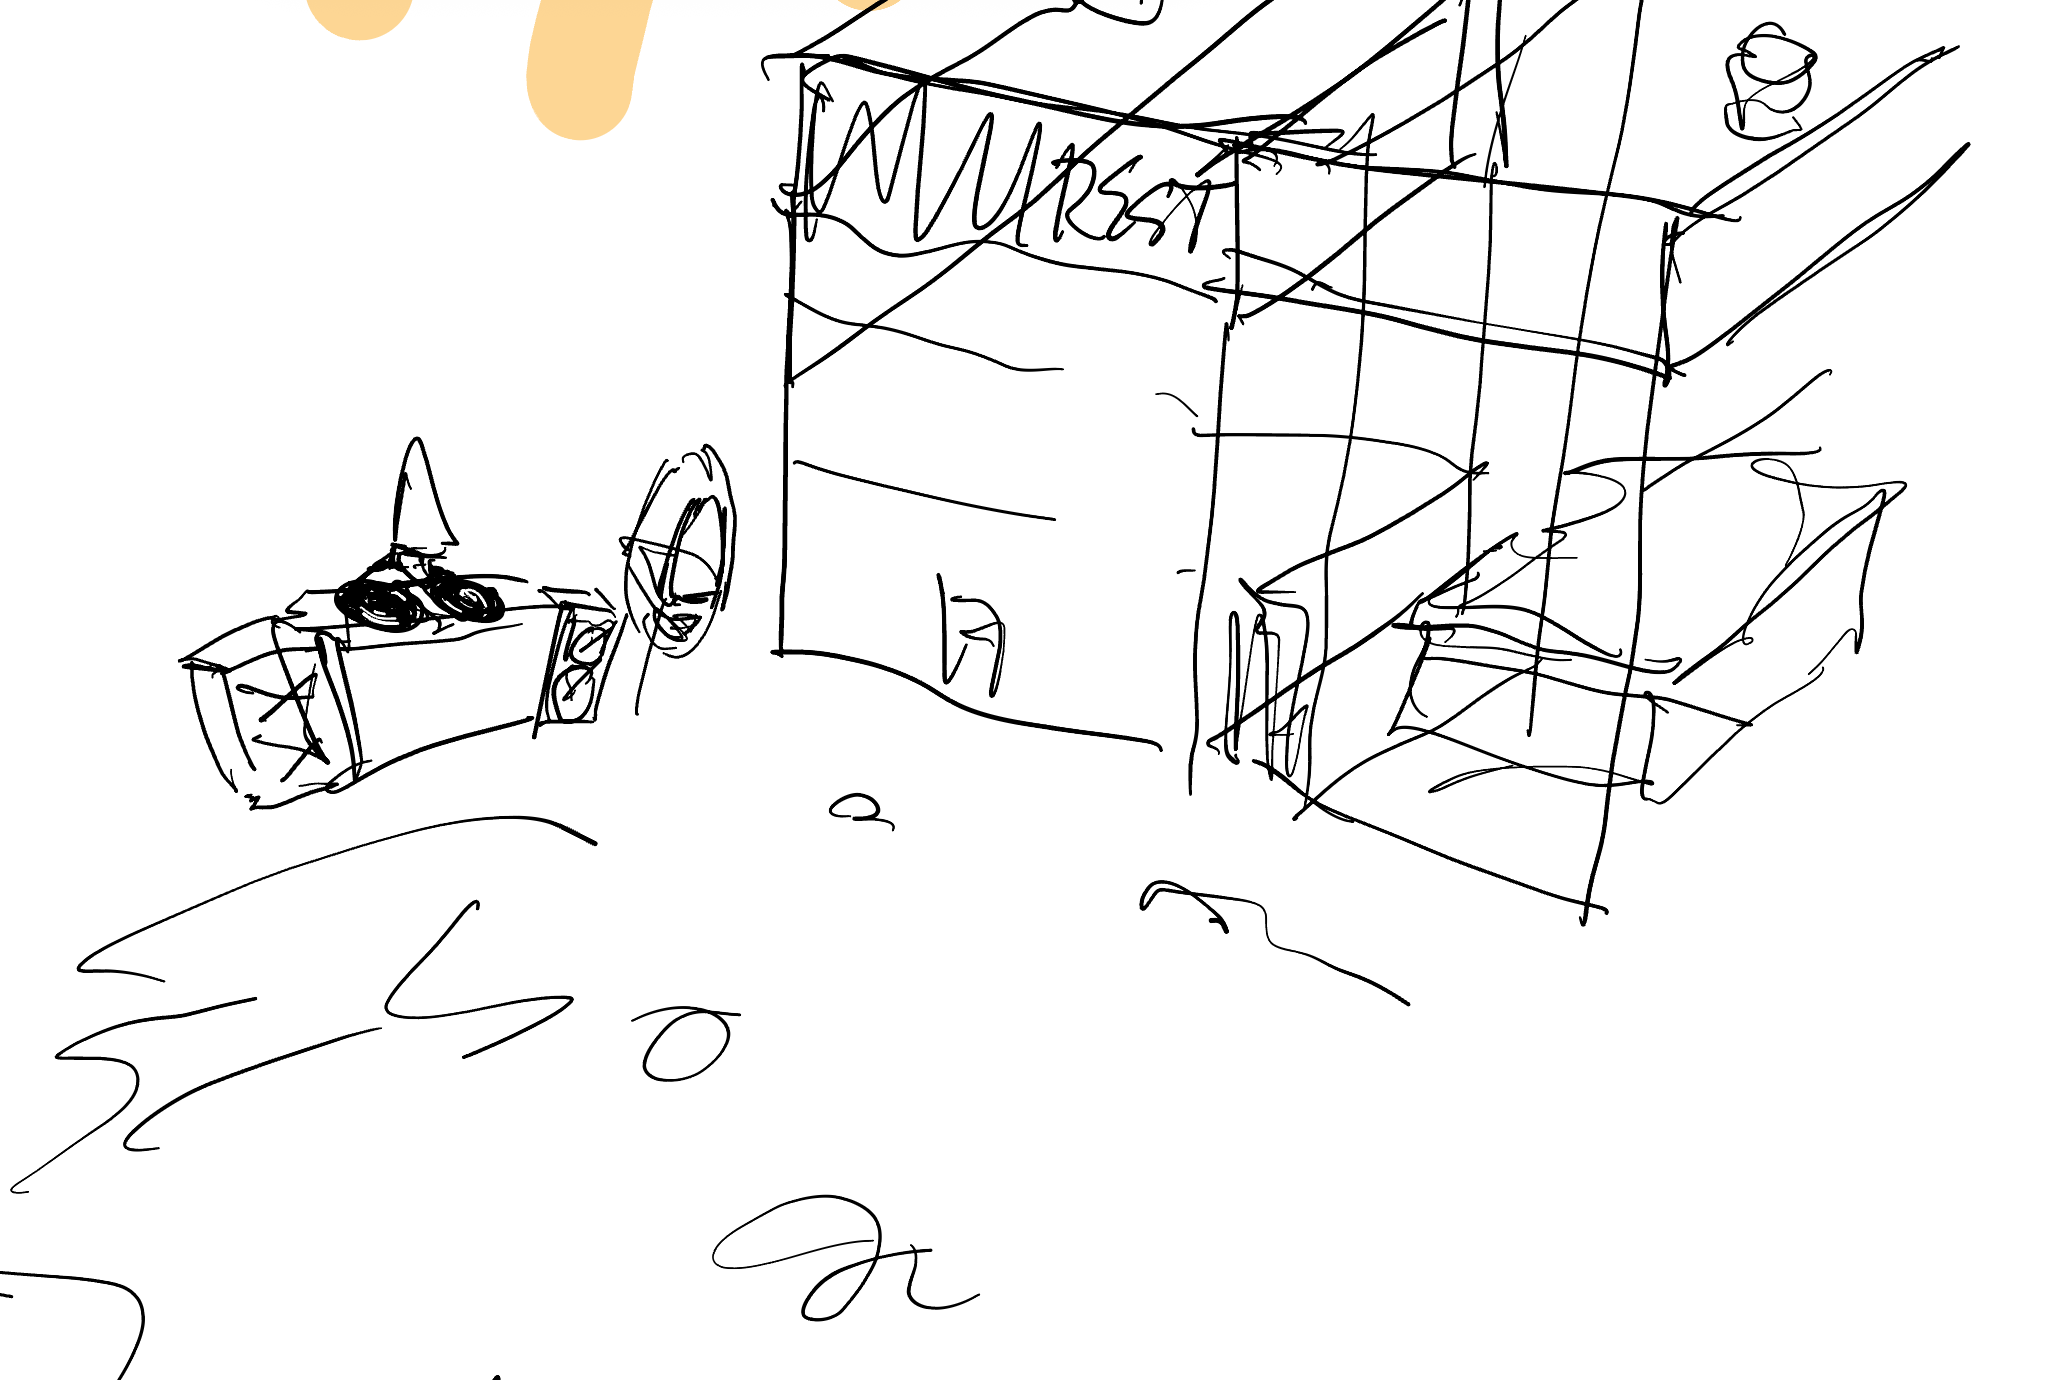
\includegraphics[width=49mm,height=31mm]{../../assets/exhibition_frames/01_entry.png}};
    \node[anchor=south west,inner sep=0,draw=signal,line width=.45pt,rotate=2]
      at (42,68) {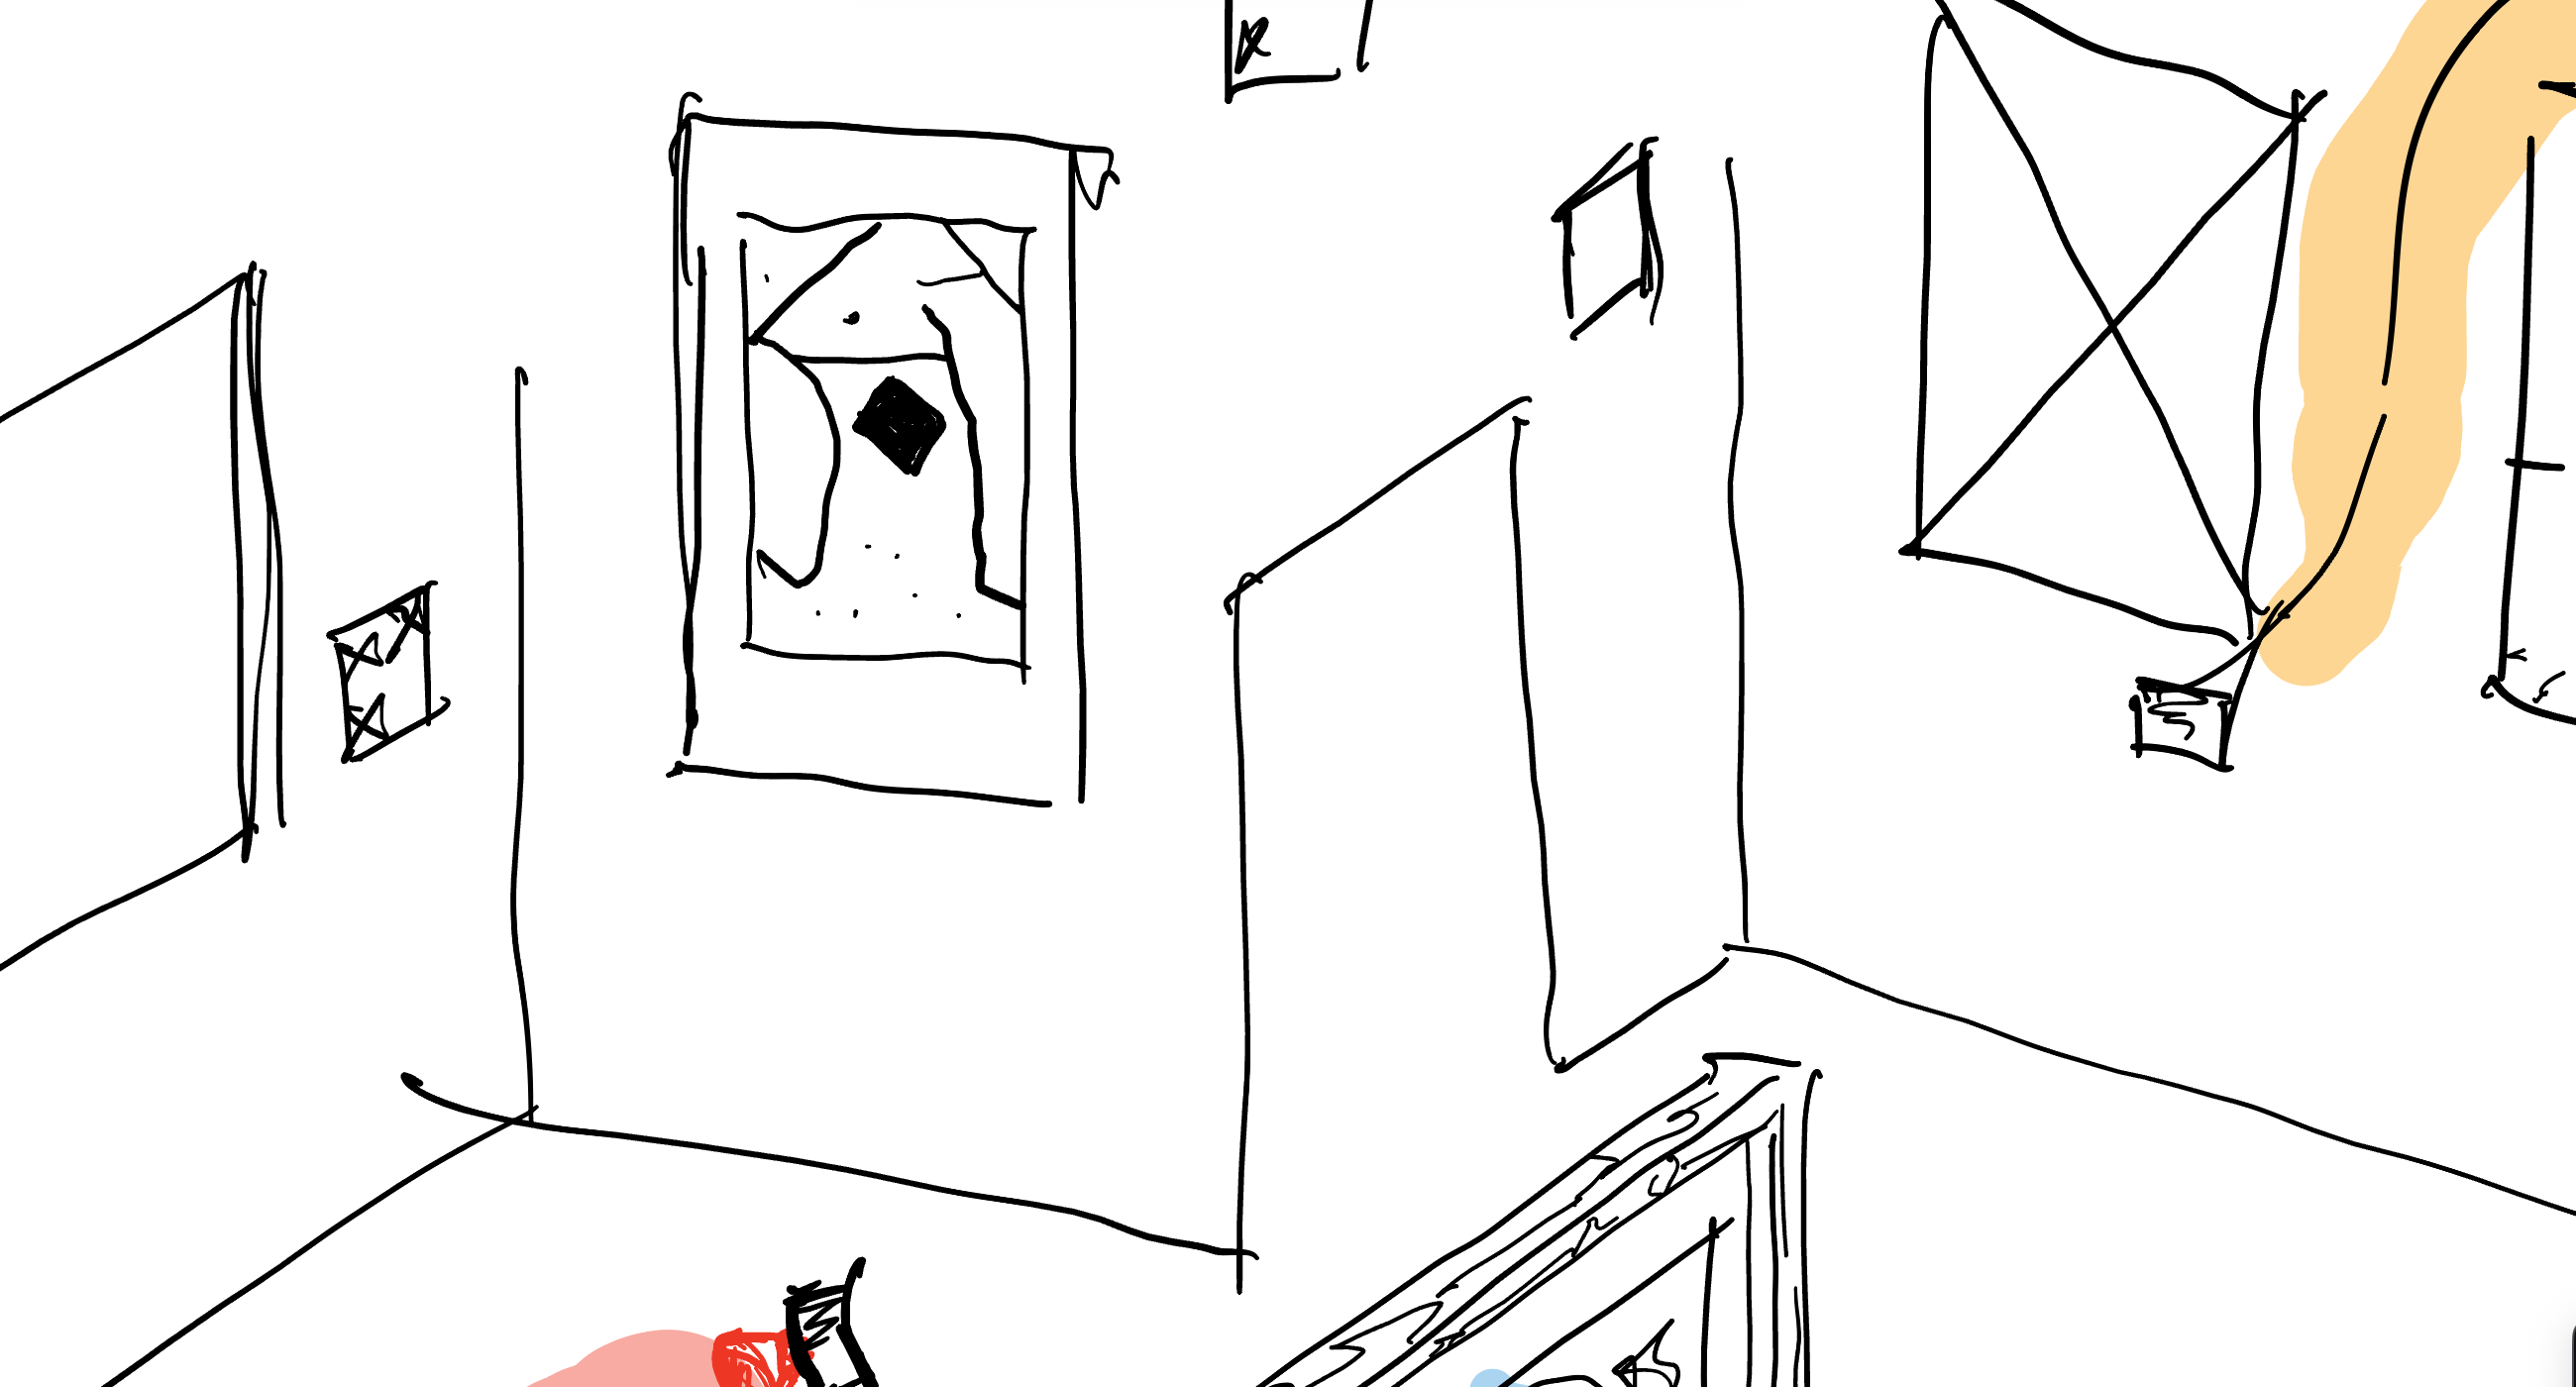
\includegraphics[width=52mm,height=30mm]{../../assets/exhibition_frames/02_wall.png}};
    \node[anchor=south west,inner sep=0,draw=signal,line width=.45pt,rotate=-1]
      at (88,57) {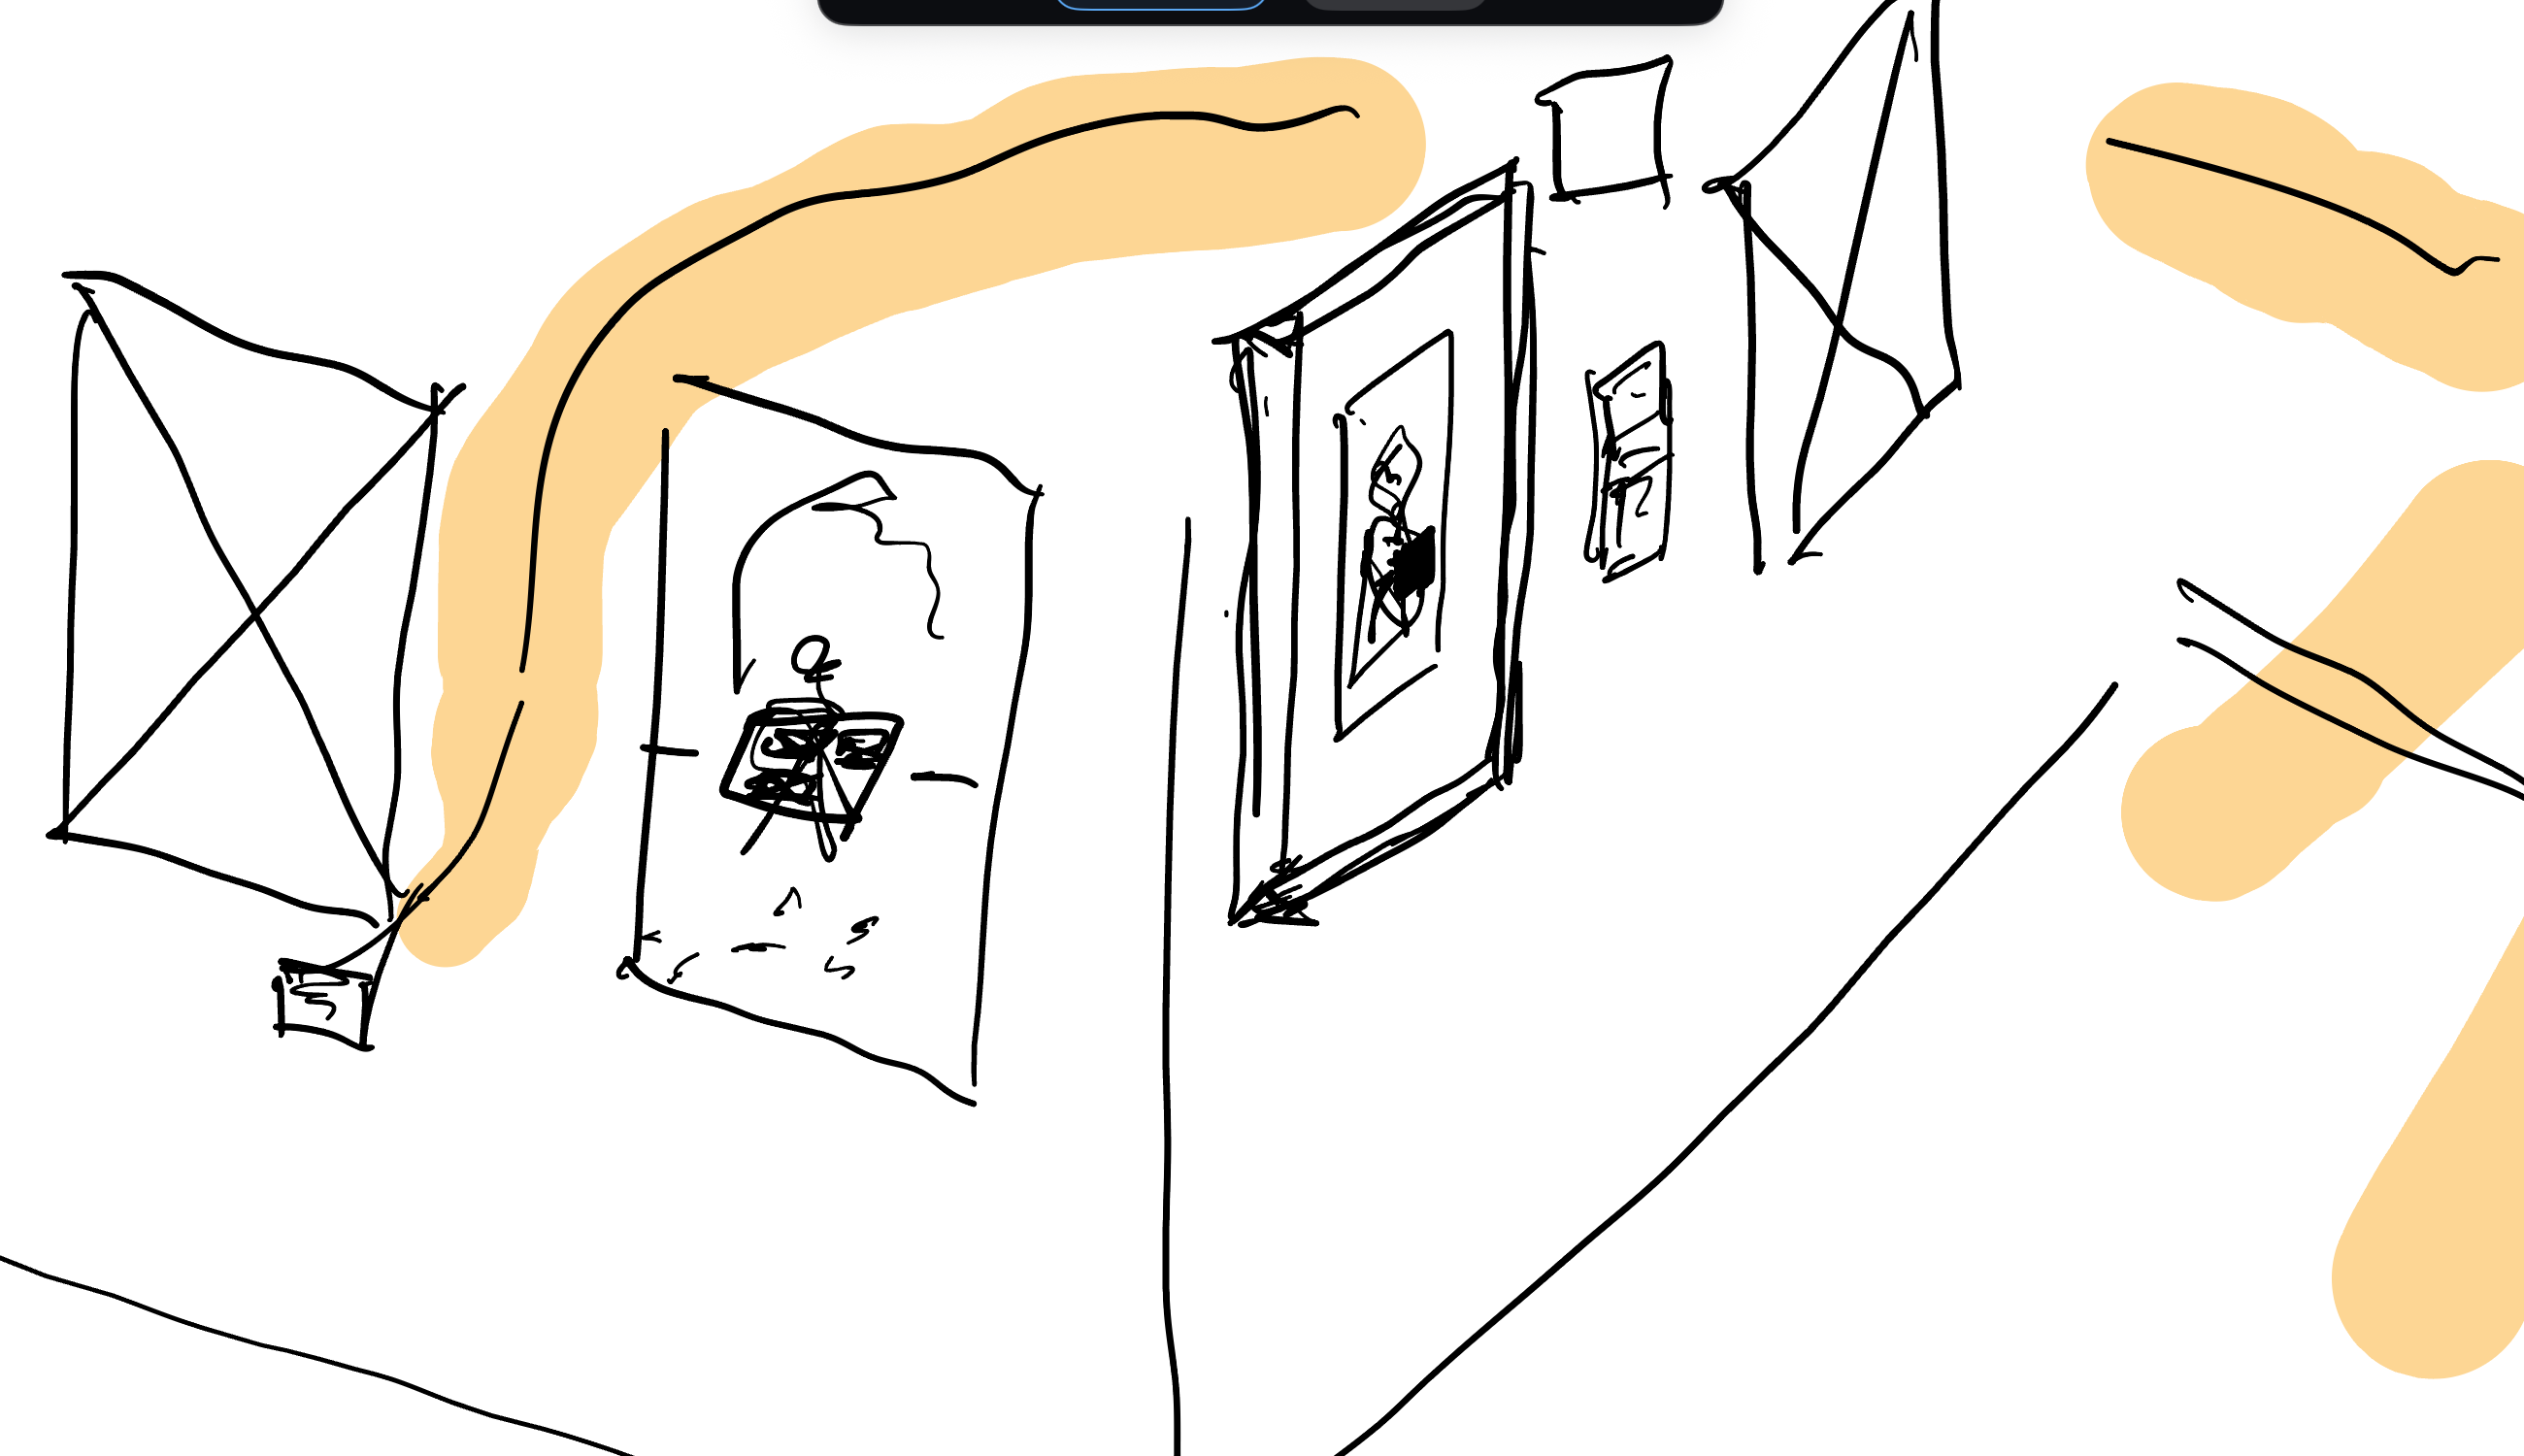
\includegraphics[width=52mm,height=32mm]{../../assets/exhibition_frames/03_turn.png}};
    \node[anchor=south west,inner sep=0,draw=signal,line width=.45pt,rotate=2]
      at (132,68) {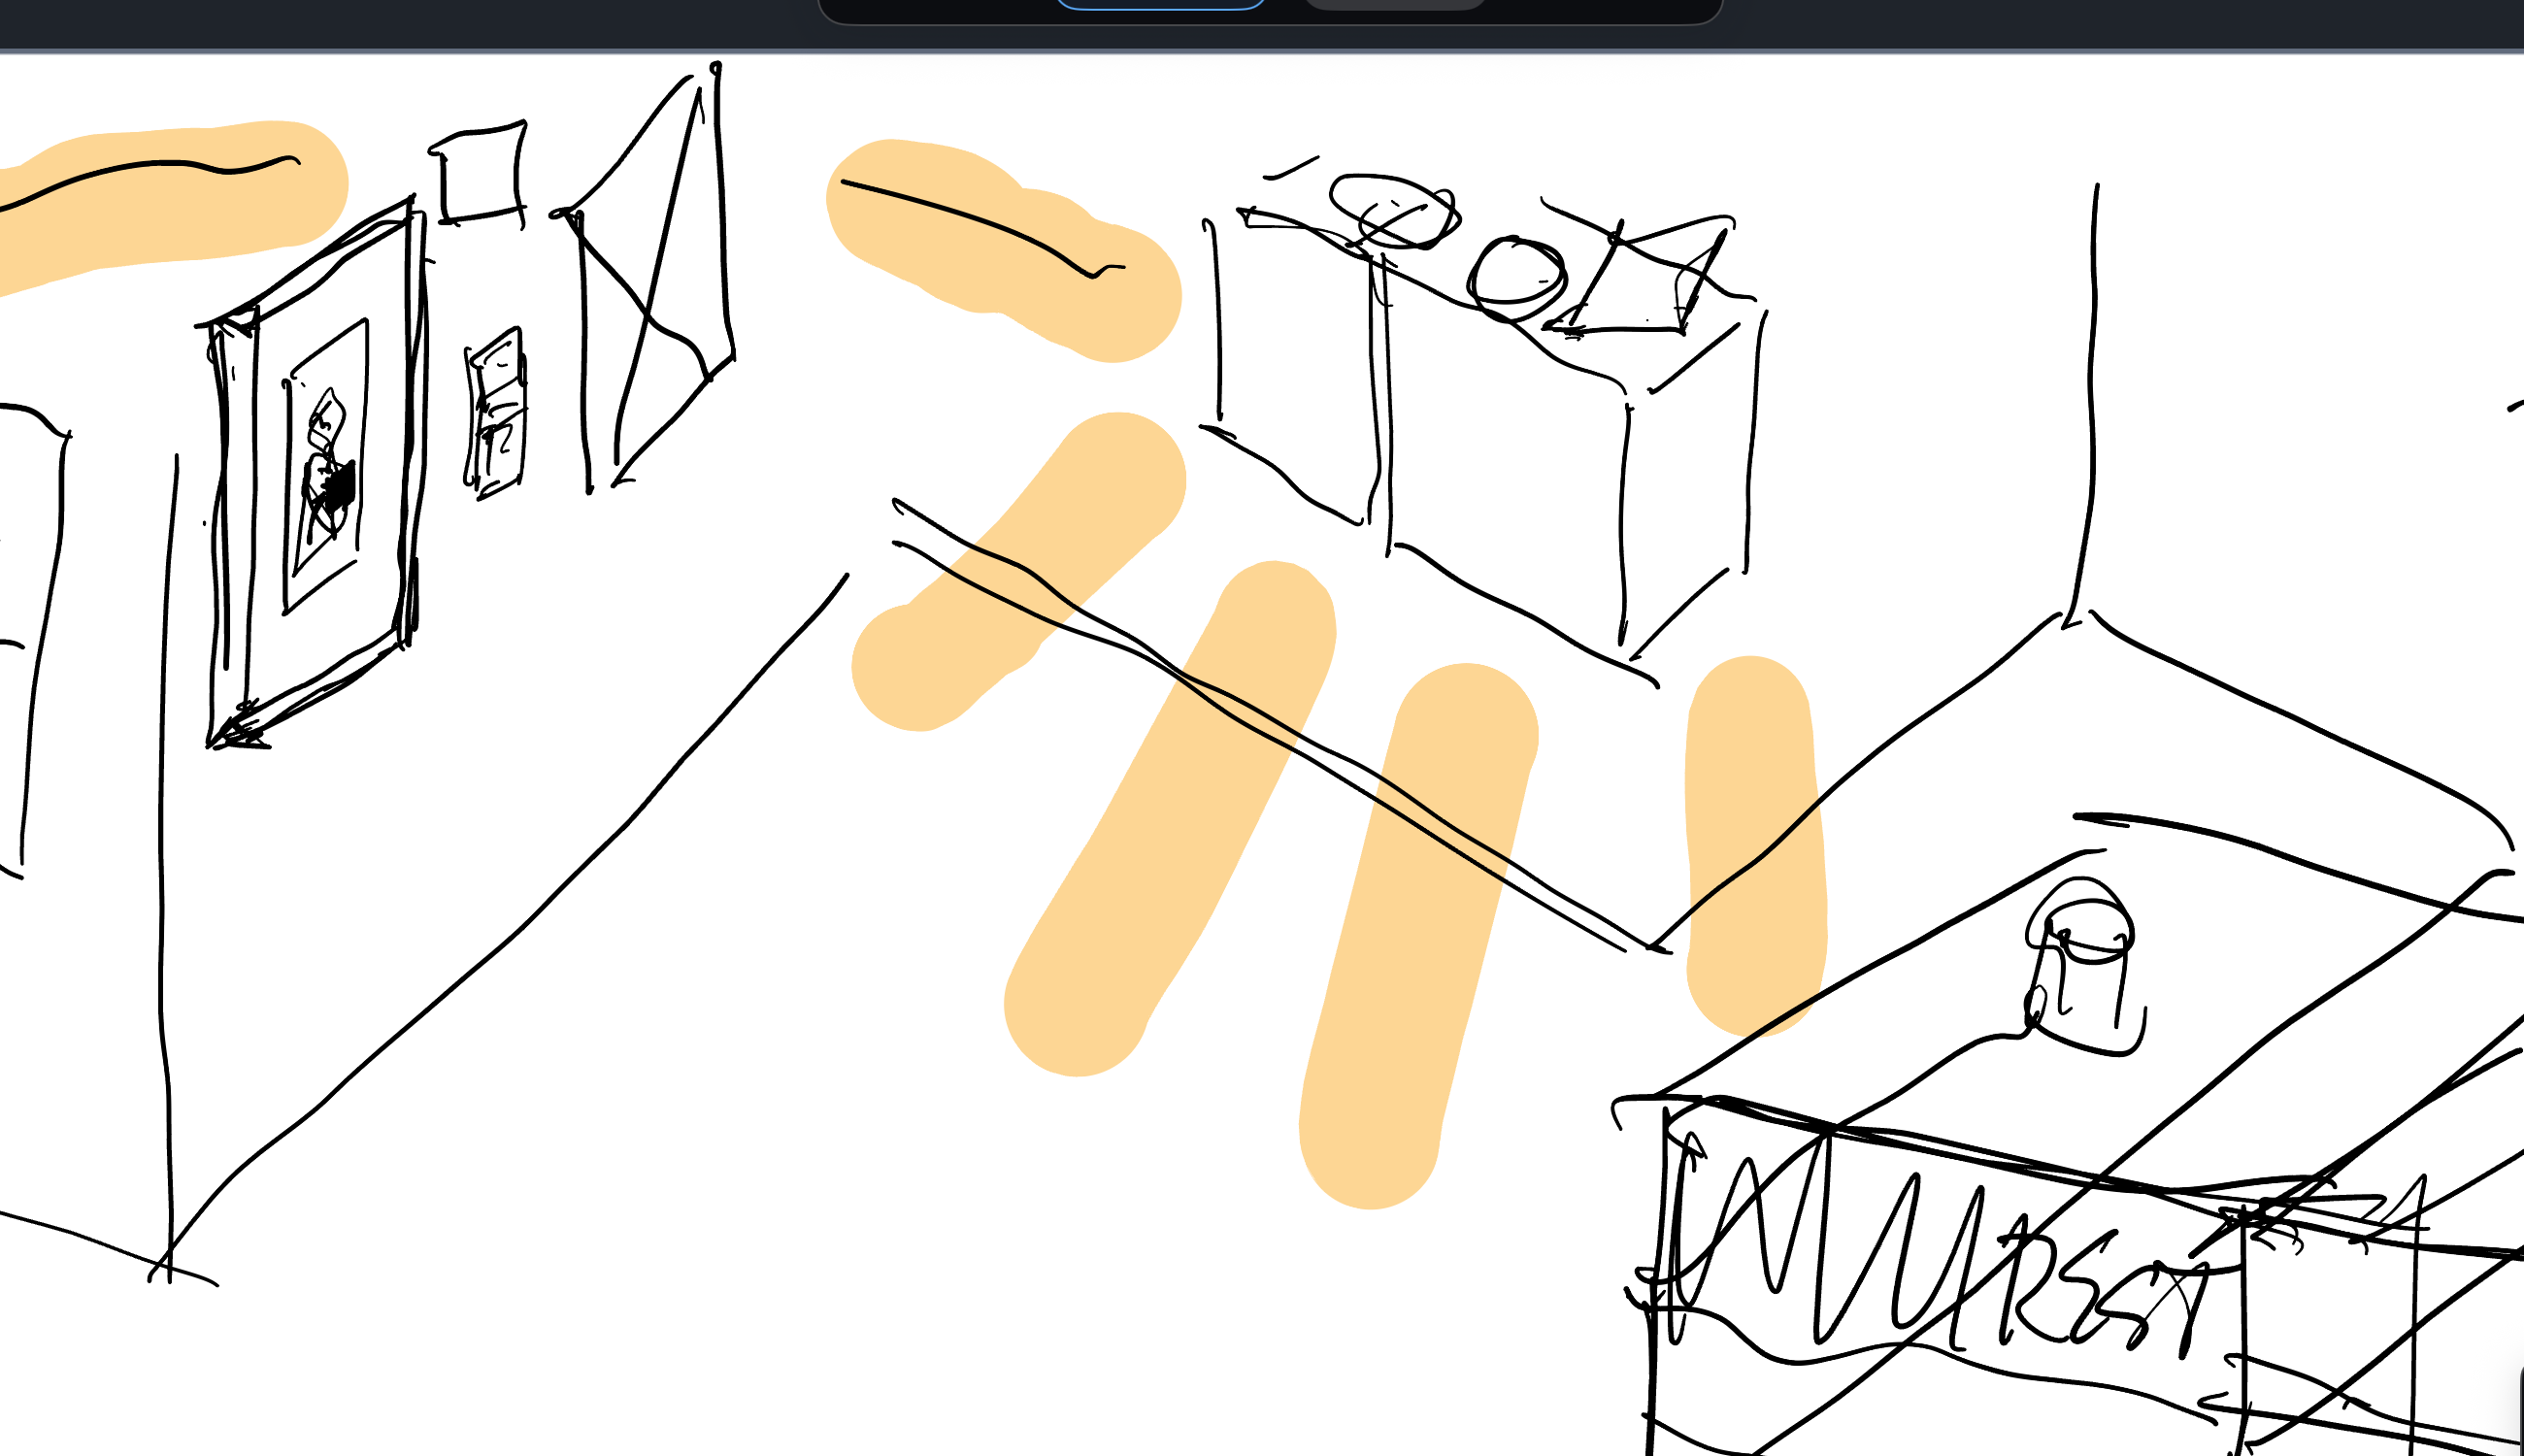
\includegraphics[width=48mm,height=30mm]{../../assets/exhibition_frames/04_field.png}};
    \node[anchor=south west,inner sep=0,draw=signal,line width=.45pt,rotate=-2]
      at (125,25) {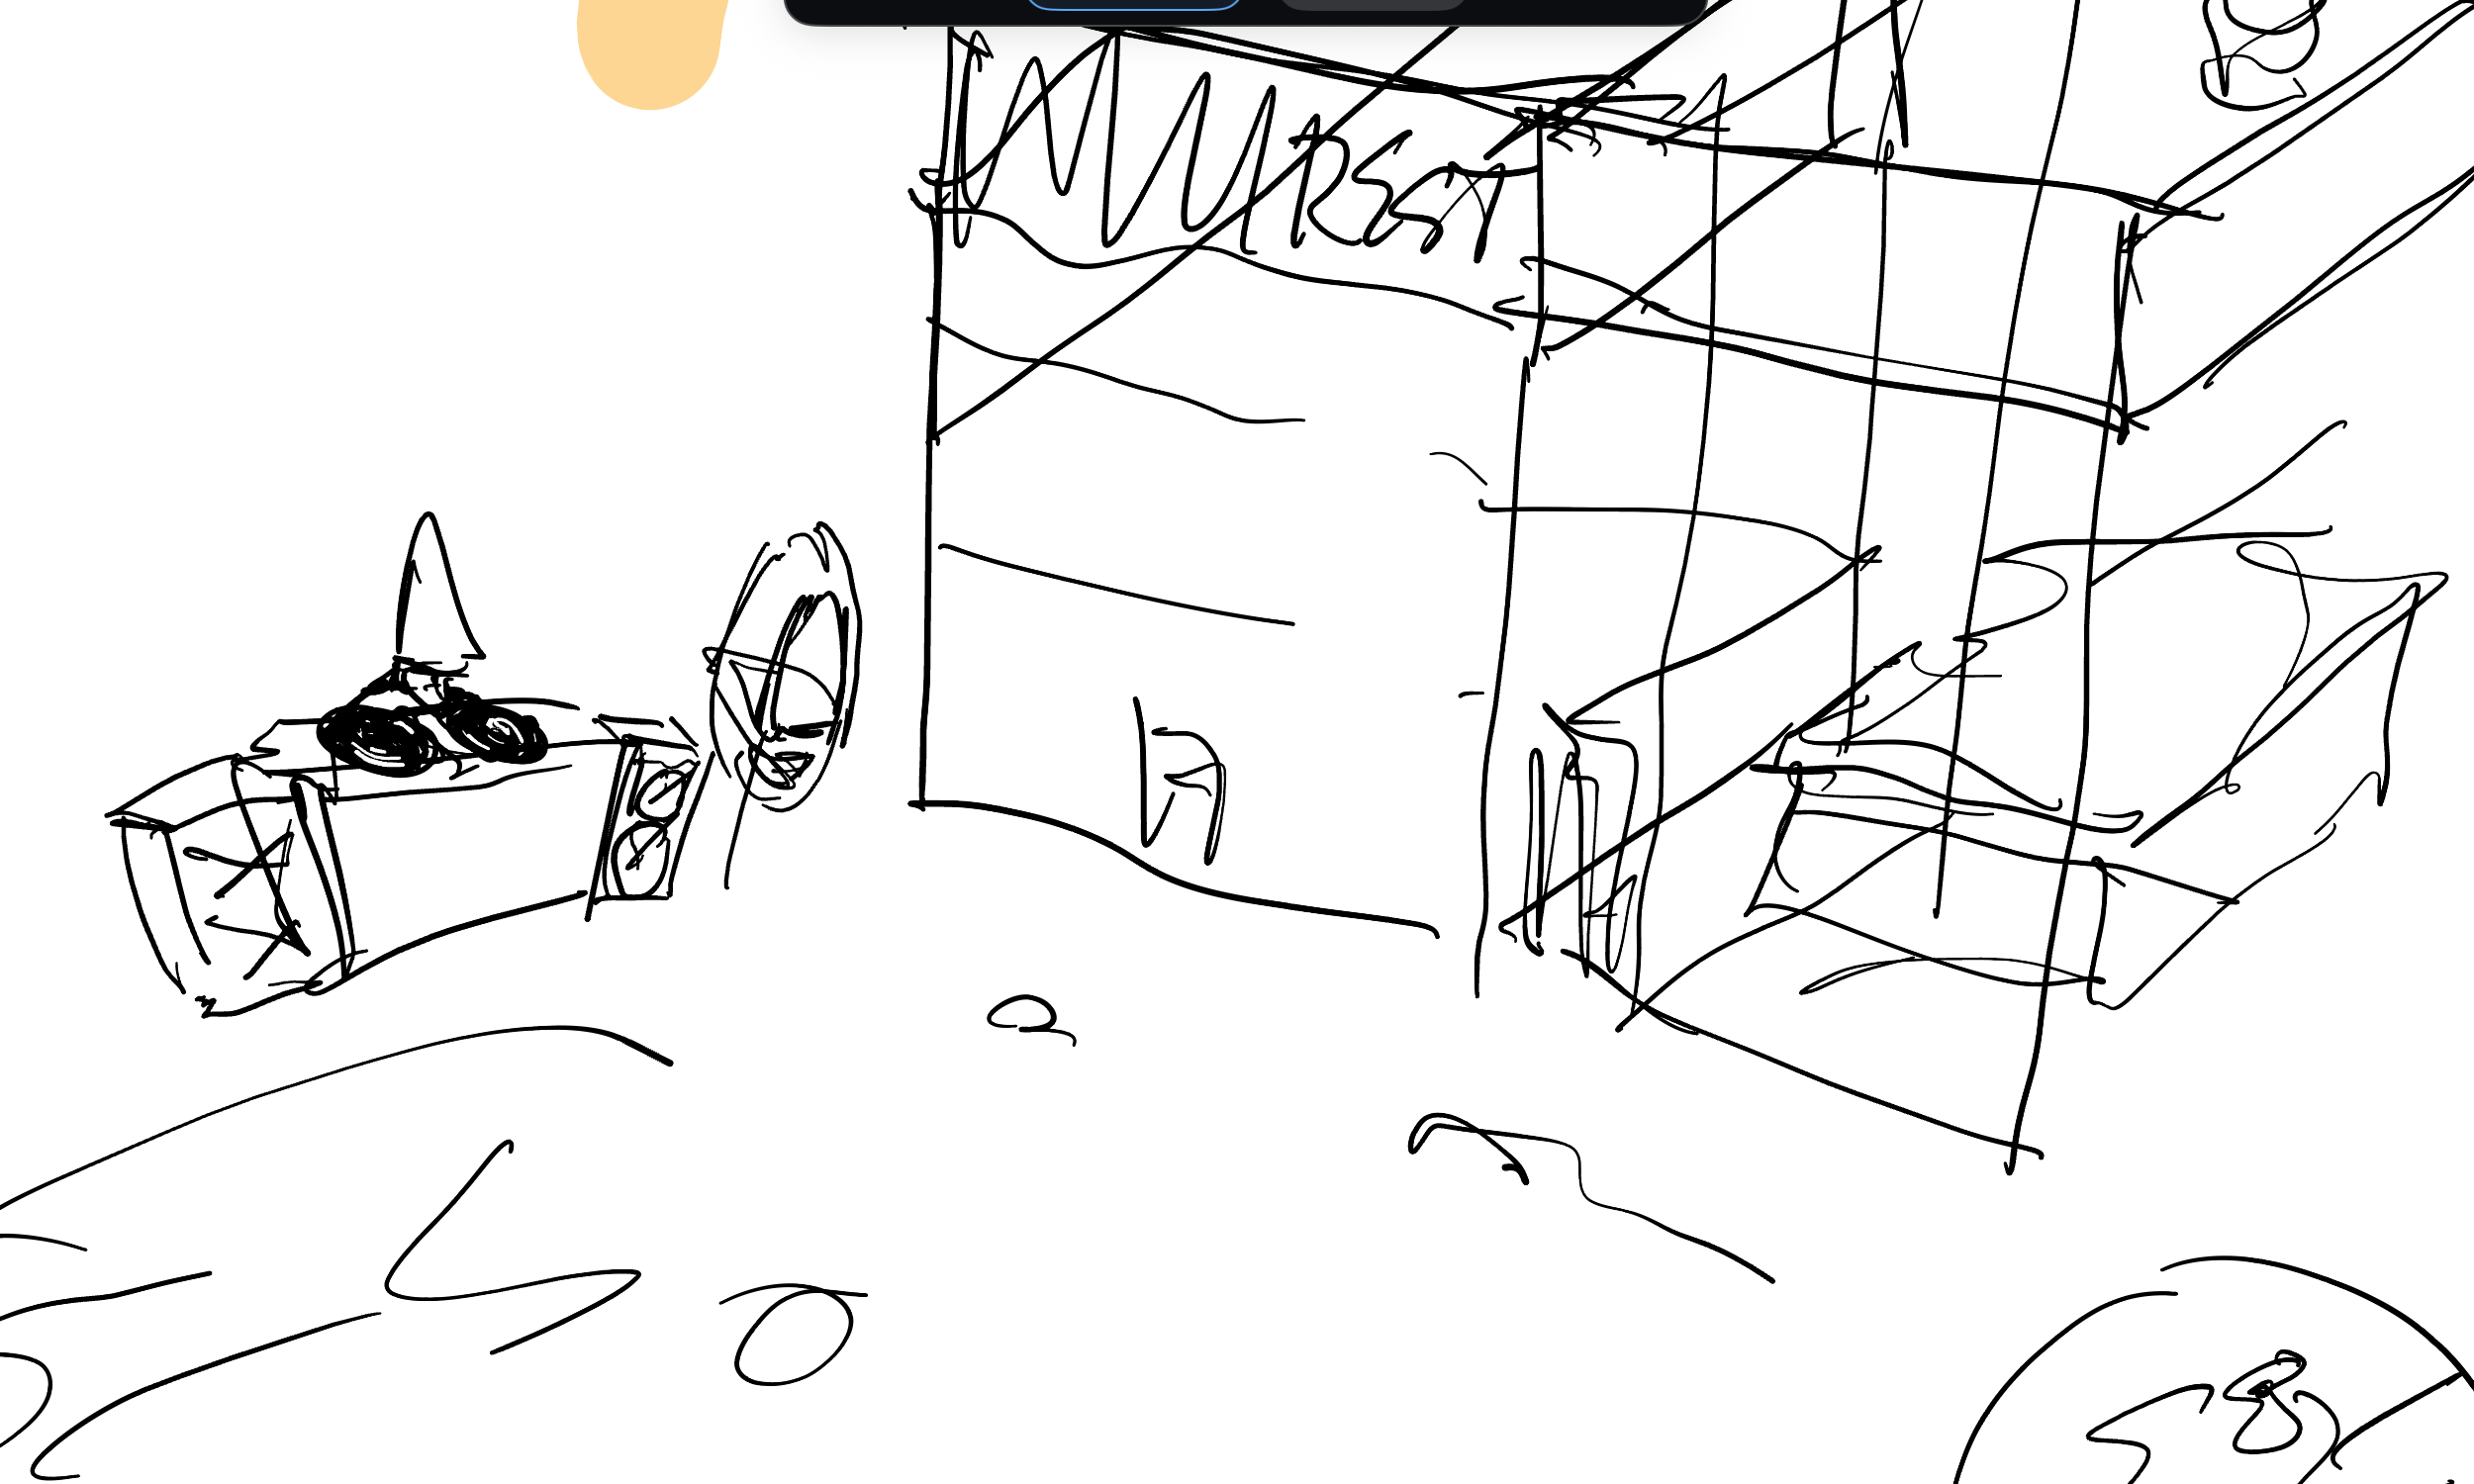
\includegraphics[width=52mm,height=32mm]{../../assets/exhibition_frames/05_return.png}};
    \node[anchor=south west,inner sep=0,draw=signal,line width=.45pt,rotate=1]
      at (68,12) {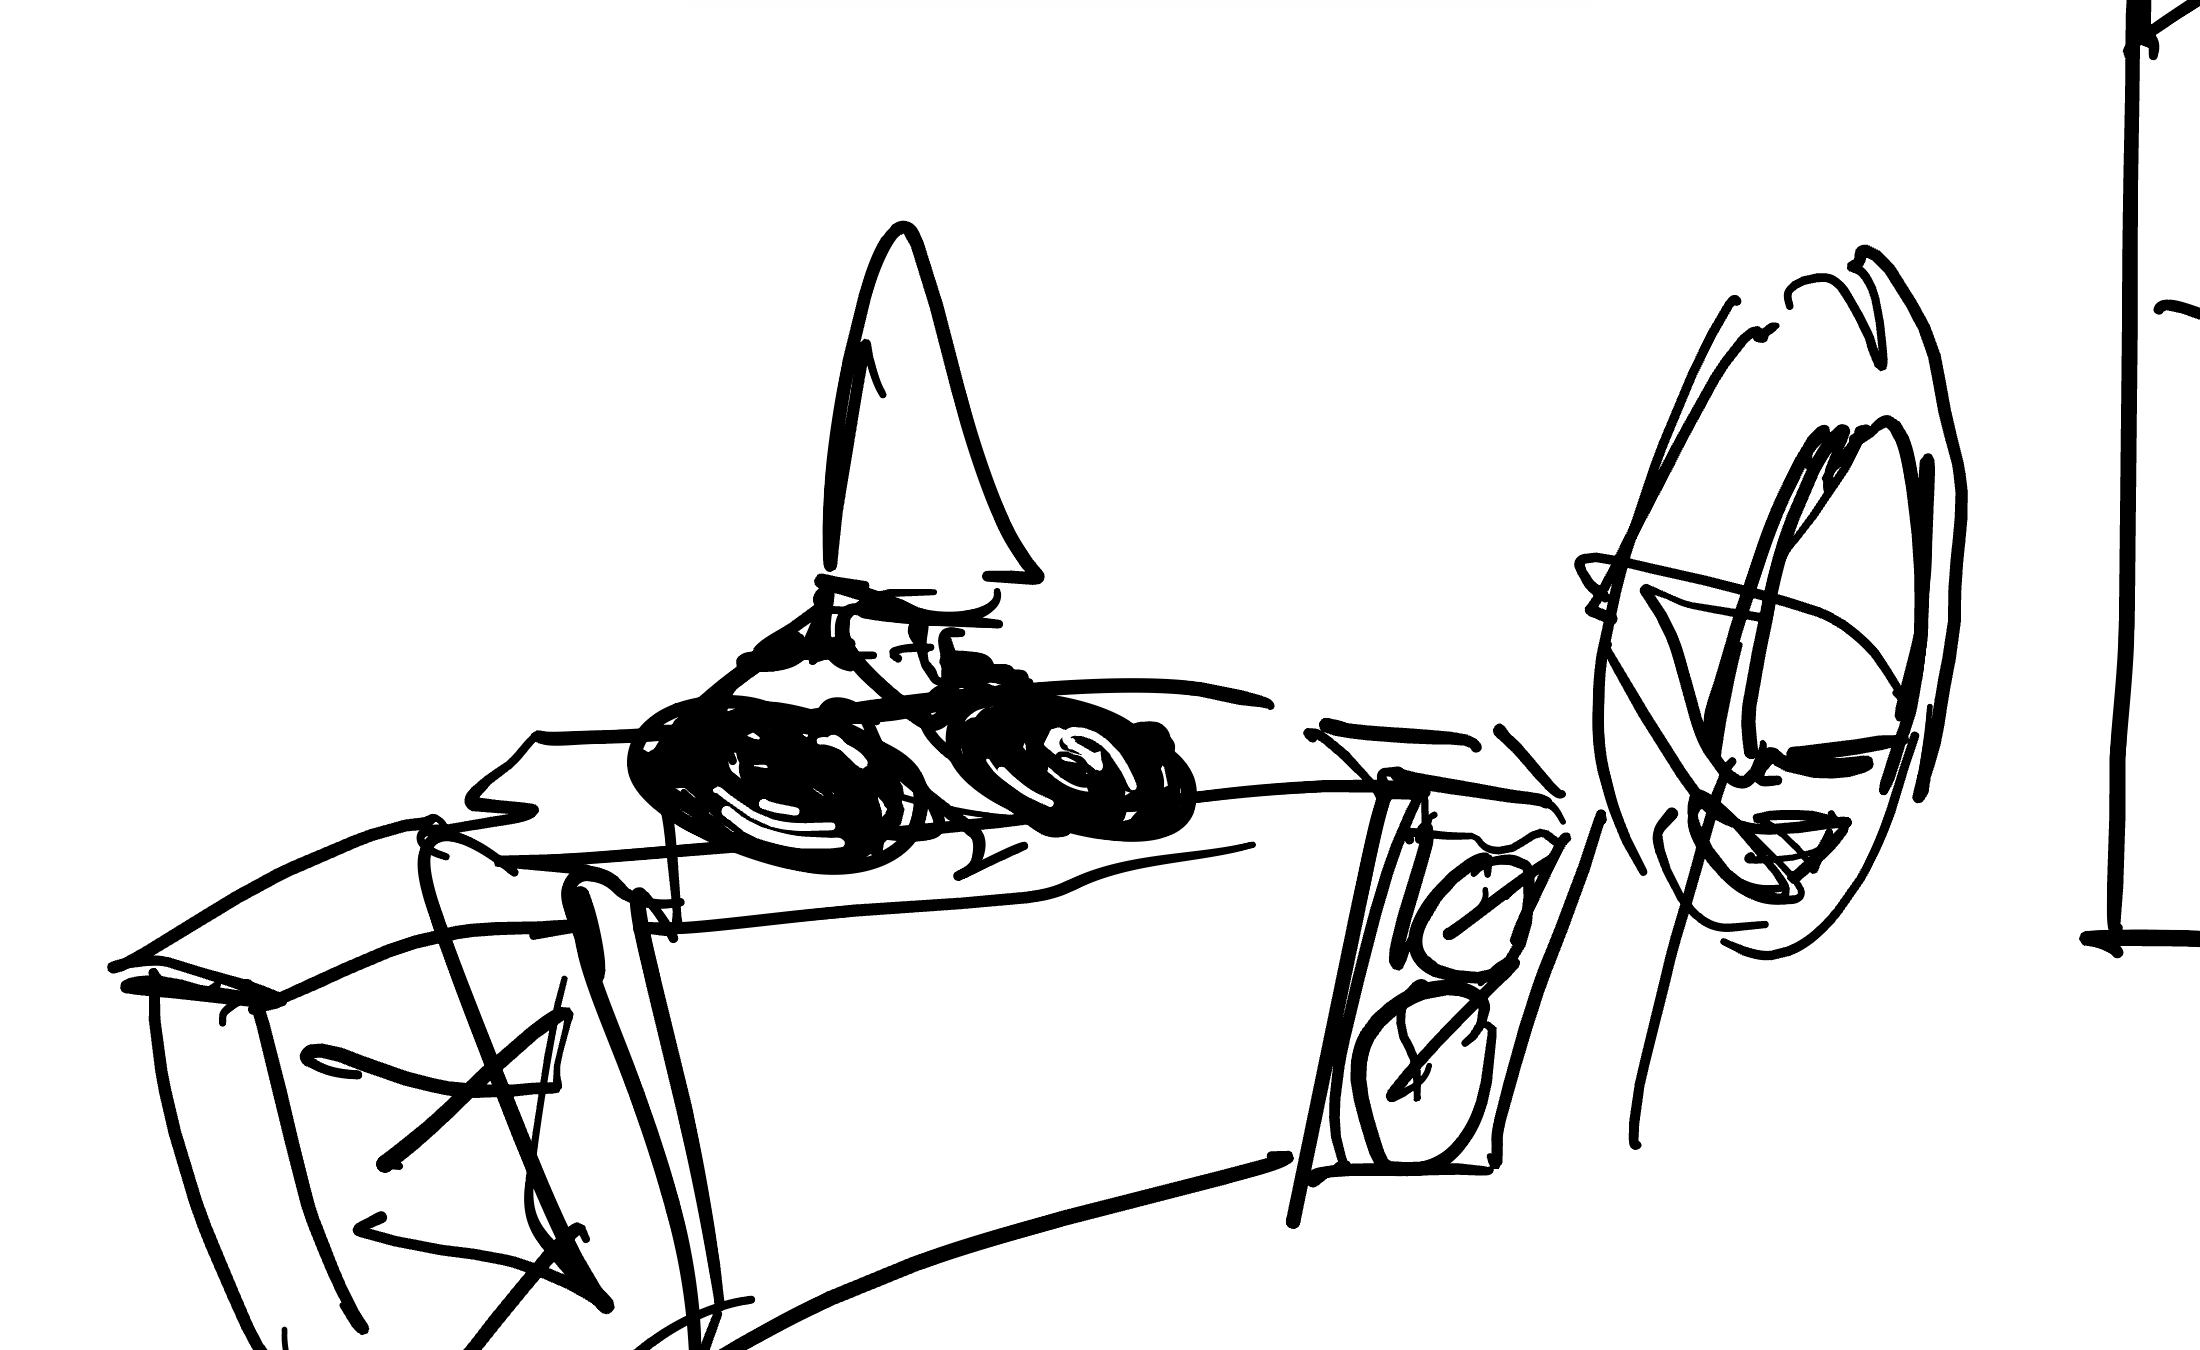
\includegraphics[width=60mm,height=37mm]{../../assets/exhibition_frames/06_sound.png}};
    \node[anchor=south west,inner sep=0,draw=signal,line width=.45pt,rotate=-1]
      at (5,20) {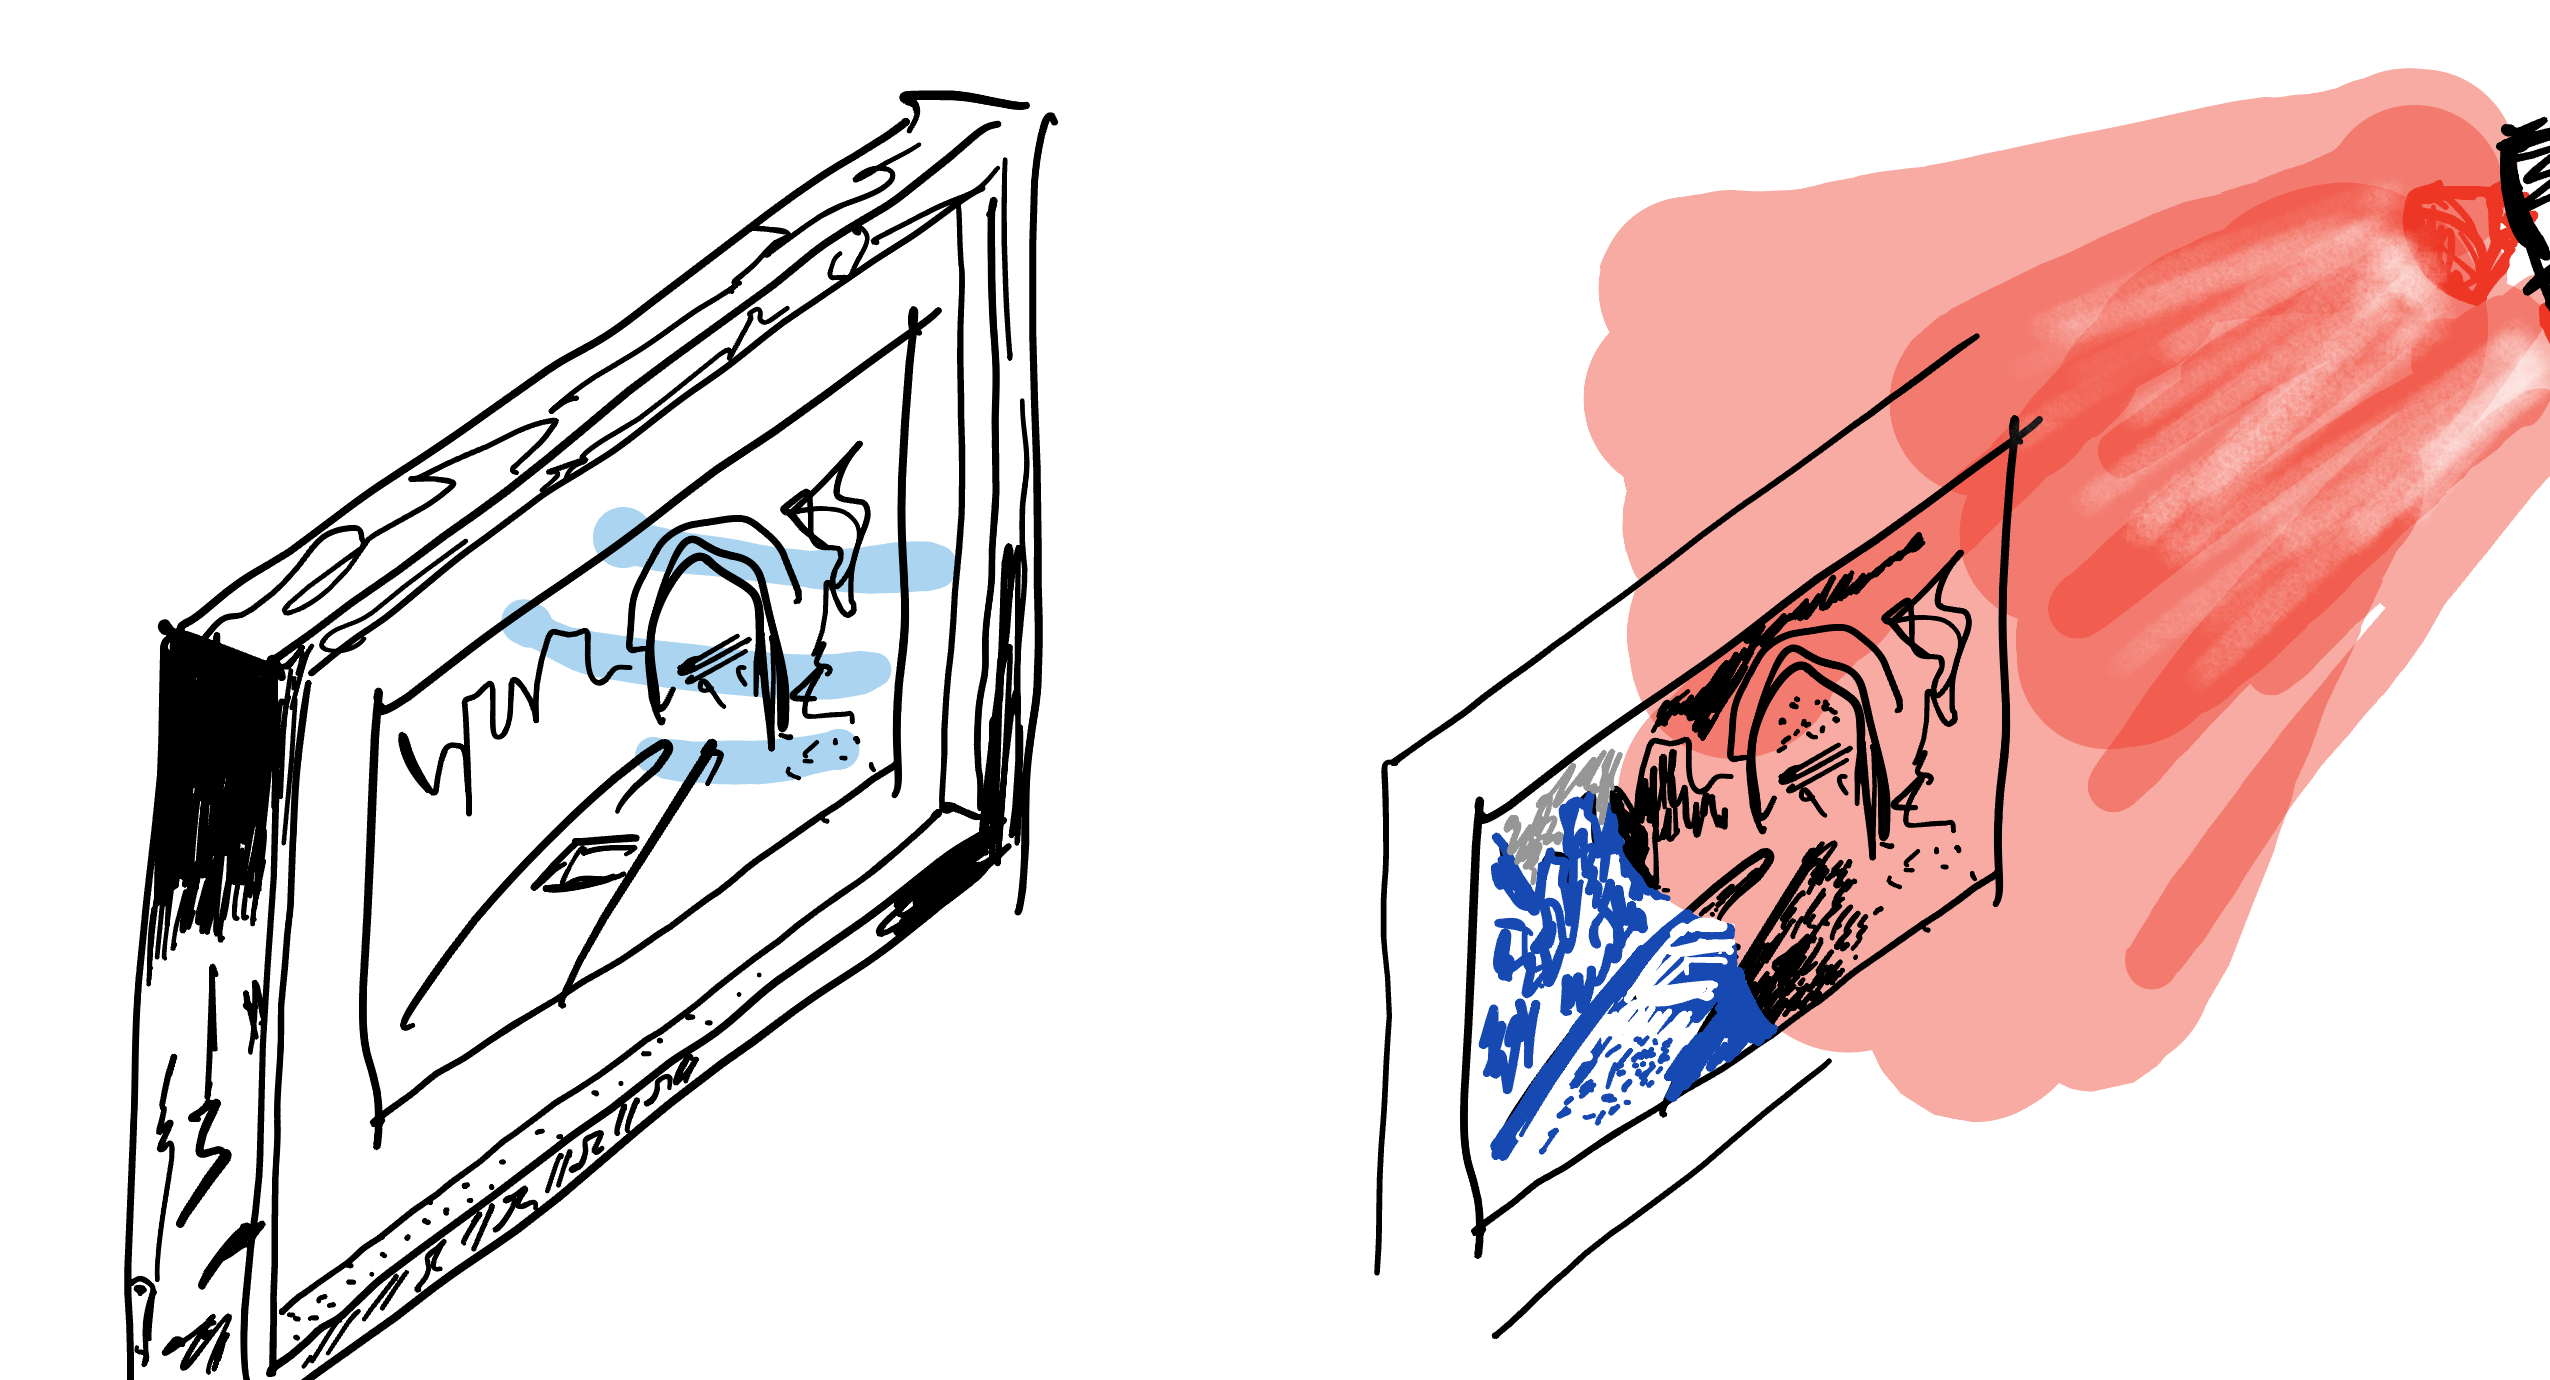
\includegraphics[width=66mm,height=38mm]{../../assets/exhibition_frames/07_projection.png}};

    \foreach \xa/\ya/\xb/\yb in {24/73/68/83,68/83/114/73,114/73/156/83,
                                   156/83/151/41,151/41/98/30,98/30/38/39}{
      \draw[white,line width=2.2pt] (\xa,\ya)--(\xb,\yb);
      \draw[signal,line width=.65pt,->] (\xa,\ya)--(\xb,\yb);
    }

    \foreach \x/\y/\n in {1/87/01,43/96/02,89/87/03,133/96/04,126/55/05,69/47/06,6/56/07}
      \node[anchor=north west,fill=black,text=white,inner sep=1.4mm,
            font=\metafont\fontsize{6.5}{7}\selectfont] at (\x,\y) {\n};
  \end{tikzpicture}\par
  \vspace{3mm}
  \smallcapsline{Fig. 1 / Propagation through wall, passage, sound, and projected image.}
\end{minipage}
\newpage

% 5 PHOTO
\meta{PHOTOGRAPH}{NODE 01}\folio{08}\sidelegend
\vspace*{36mm}\hspace*{14mm}
\begin{minipage}{179mm}
  \photobox[205mm]{kumiori / ABANDONED CHURCH / SELECTED SEQUENCE}
  \vspace{4mm}
  \smallcapsline{Architectures / bodies / apertures / objects / frame to frame.}
\end{minipage}
\newpage

% 6 VOICE
\meta{VOICE}{NODE 01 / AUDIO}\folio{09}\sidelegend
\vspace*{47mm}\hspace*{62mm}
\begin{minipage}{\mainmeasure}
  \statement{IMAGE IS NOT\\ENOUGH TO CARRY.}\par
  \vspace{28mm}
  \hfill\begin{minipage}{70mm}\centering
    \qrprogression{inv_qr_04_de54.png}{inv_qr_05_2270.png}{inv_qr_06_3863.png}%
      {04--06 / STRUCTURE EMERGING}\par\vspace{3mm}
    \smallcapsline{LISTEN}
  \end{minipage}
\end{minipage}
\begin{tikzpicture}[remember picture,overlay]
  \node[anchor=south east,align=left,text width=72mm]
    at ([xshift=-18mm,yshift=22mm]current page.south east) {%
      {\relationfont\fontsize{10.5}{13}\selectfont\itshape
      Mai-Brit Tänava enters through recorded voice. The QR portal opens
      another perspective from inside the frame.}%
    };
\end{tikzpicture}
\newpage

% 7 MULTIPLEX
\meta{SYSTEM}{MULTIPLEX}\folio{10}\sidelegend
\vspace*{45mm}\hspace*{62mm}
\begin{minipage}{\mainmeasure}
  \sectionnumber{1}\par\vspace{1mm}
  {\RaggedRight\displayfont\color{signal}\fontsize{23}{24}\selectfont WHAT GROWS BETWEEN THEM\\IS THE WORK.}\par
  \vspace{12mm}
  {\color{signal}\fontsize{17}{25}\selectfont\boldmath
    \[
      \begin{aligned}
      &\boldsymbol{\mathcal W_t=\{w_1,w_2,\ldots,w_n\}},\\
      &\boldsymbol{\mathcal R_t\subseteq\mathcal W_t\!\times\!\mathcal W_t},\\
      &\boldsymbol{\mathcal G_t=(\mathcal W_t,\mathcal R_t)}.
      \end{aligned}
    \]}
  \vspace{12mm}
  {\fontsize{10.8}{14}\selectfont
  $\mathcal W_t$ is the set of attributable contributions present at time $t$:
  images, voices, sounds, bodies, places, and practices. $\mathcal R_t$ is not
  subtraction and not another object. It is a set of ordered pairs. Writing
  $(w_i,w_j)\in\mathcal R_t$ means that an encounter lets $w_i$ alter the possible
  continuation of $w_j$. The relation can be added, changed, or removed; therefore
  $\mathcal R_t$ is not fixed in advance. $\mathcal G_t$ names the state of TAKE OVER
  at that moment: distinct contributions together with the relations currently
  active between them.\par\vspace{5mm}

  \textbf{Attributable authors, ordered alphabetically by surname:}
  Kenn-Eerik Kannike; Andrés A. León Baldelli / kumiori III; Ave Palm; and
  Mai-Brit Tänava. Their contributions remain distinct while entering relation.}

  \vspace{12mm}
  {\relationfont\fontsize{14}{18}\selectfont\itshape
    Take over the wall.\par
    Take over the oven.\par
    Take over the sound.\par
    Take over the restaurant.\par
    Take over the night.\par
    Take over the surface.\par}
\end{minipage}
\newpage

% 8 EMPTY
\meta{VACANCY}{OPEN NODE}\folio{11}\sidelegend
\vspace*{54mm}\hspace*{14mm}
\begin{minipage}{179mm}
  \statement{UNALLOCATED\\IS NOT EMPTY.}\par
  \vspace{92mm}
  {\fontsize{18}{23}\selectfont\itshape Not because material is missing. Because somebody is.}\par
  \vspace{12mm}
  {\fontsize{34}{42}\selectfont\[\mathrm{WHO\ ENTERS\ NEXT?}\]}
\end{minipage}
\newpage

% 9 PHOTO 2
\meta{PHOTOGRAPH}{NODE 02}\folio{12}\sidelegend
\vspace*{36mm}\hspace*{14mm}
\begin{minipage}{180mm}
  \photobox[205mm]{AVE PALM / PROVISIONAL SELECTION}
  \vspace{4mm}
  \smallcapsline{Abandoned architectures / bodies / movement / cyanotype.}
\end{minipage}
\newpage

% 10 SOUND
\meta{SOUND}{NODE 03}\folio{13}\sidelegend
\begin{tikzpicture}[remember picture,overlay]
  \node[anchor=north west,align=left,text width=38mm,
        font=\fontsize{8.5}{11}\selectfont]
    at ([xshift=14mm,yshift=-92mm]current page.north west)
    {\relationfont\textbf{ARVO P\"ART}\\[-.5mm]\textit{Ludus}\\[1.5mm]\textit{``game'' in Latin}};
\end{tikzpicture}
\vspace*{47mm}\hspace*{62mm}
\begin{minipage}{\mainmeasure}
  \bigstatement{LISTEN.}\par
  \vspace{18mm}
  {\fontsize{14}{19}\selectfont
    Sound is location and grounding. Some QR portals carry recordings made at or in relation to the photographed sites; others carry voices or composed material. Kenn-Eerik Kannike develops the sonic trajectory through recordings, listening, and live electronic concert.}
  \vspace{24mm}
  \begin{center}
    \begin{tikzpicture}[x=1cm,y=1cm]
      \node[anchor=south west,inner sep=0] at (0,0)
        {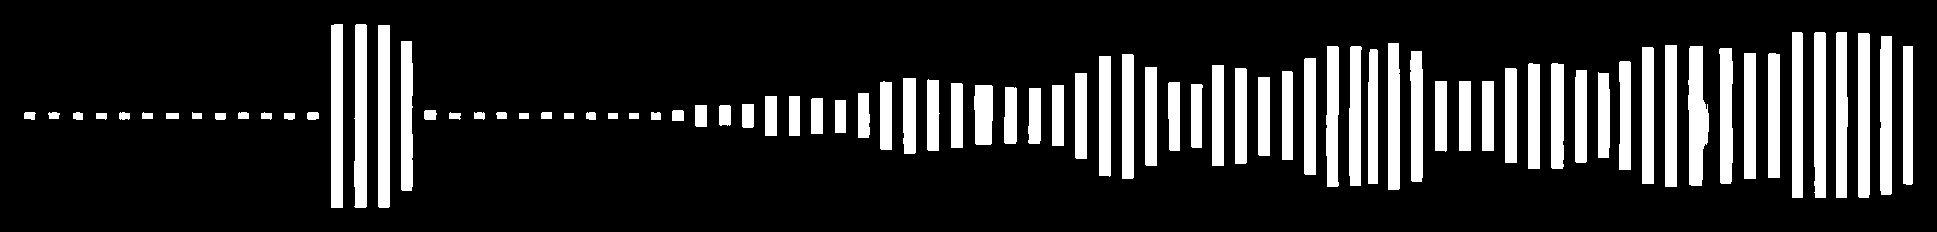
\includegraphics[width=12cm,height=1.8cm]{../../fig/listen_waveform_clean.png}};
      \node[anchor=north,text=signal,font=\metafont\fontsize{7}{9}\selectfont] at (2.05,-.35) {CHIRP};
      \node[anchor=north,text=signal,font=\metafont\fontsize{7}{9}\selectfont] at (4.85,-.35) {SILENCE};
      \node[anchor=north east,text=signal,font=\metafont\fontsize{7}{9}\selectfont] at (12,-.35) {SMOOTH CRESCENDO};
      \draw[signal,line width=.45pt] (2.05,0)--(2.05,-.9)--(0,-.9);
      \node[anchor=north west,text=signal,font=\metafont\fontsize{7}{9}\selectfont]
        at (0,-1.08) {CHIRP EVENT / SPECTRAL ZOOM};
      \node[anchor=north east,text=signal,font=\metafont\fontsize{6.2}{8}\selectfont]
        at (12,-1.08) {FREQUENCY $\uparrow$ / TIME $\rightarrow$};
      \node[anchor=south west,inner sep=0] at (0,-5.55)
        {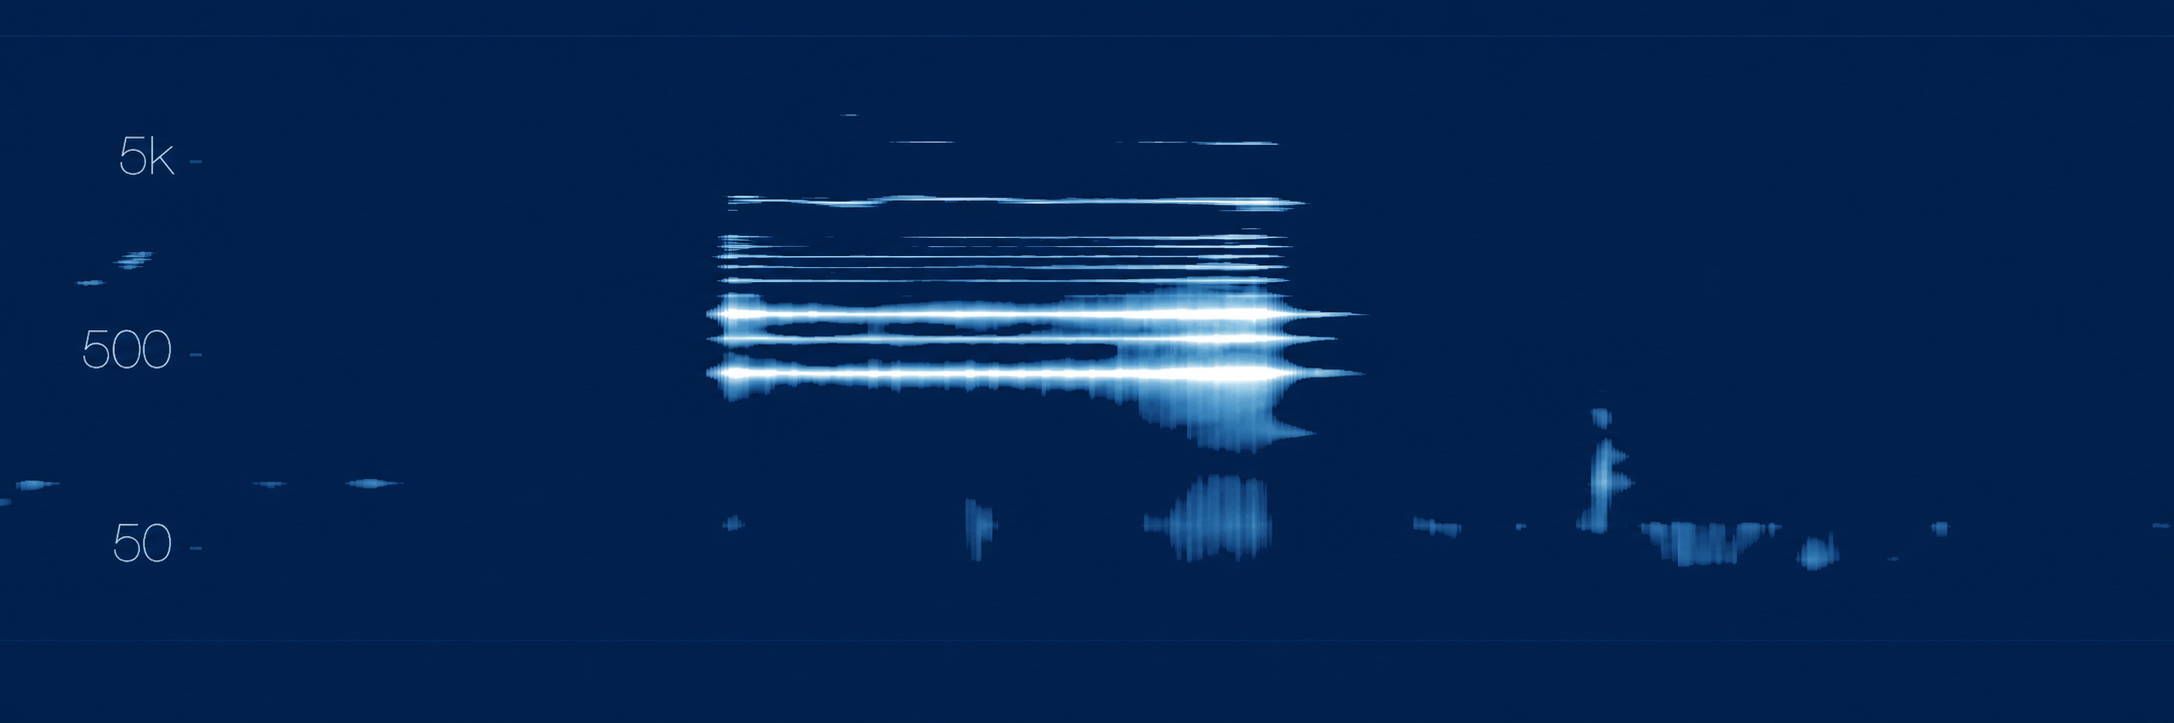
\includegraphics[width=12cm,height=3.8cm]{../../fig/arvo_paart_ludus_chirp_cyanotype.png}};
    \end{tikzpicture}
  \end{center}
\end{minipage}
\newpage

% 11 TRAJECTORY
\meta{TRAJECTORY}{TIMELINE}\folio{14}\sidelegend
\vspace*{45mm}\hspace*{62mm}
\begin{minipage}{\mainmeasure}
  \sectionnumber{2}\par\vspace{1mm}
  {\RaggedRight\displayfont\color{signal}\fontsize{23}{24}\selectfont THE OPENING CHANGES\\THE EXHIBITION.}\par
  \vspace{24mm}
  \begin{tikzpicture}[x=1mm,y=1mm]
    \draw[signal,line width=.8pt] (0,0)--(121,0);
    \foreach \x/\lab in {1/APPLY,28/HUMAN,59/OPENING,91/NIGHT,121/?}{\fill[signal] (\x,0) circle (1.7pt);\node[anchor=north,text=signal,font=\metafont\fontsize{6.5}{8}\selectfont] at (\x,-4) {\lab};}
    \draw[signal,dashed,line width=.5pt] (59,-18)--(59,38);
    \node[anchor=south west,align=left,text width=50mm,font=\fontsize{11}{14}\selectfont] at (61,10) {photography $+$ voice $+$\\situated sound $+$ movement};
  \end{tikzpicture}
  \vspace{34mm}
  {\fontsize{12}{16}\selectfont Concert, live sound, performance, food, and night are possible consequences, not requirements. Each practice enters as someone brings it. Something happens. There is an interval. What follows is changed by it.}
\end{minipage}
\newpage

% 12 NEEDS
\meta{NECESSITIES}{CURRENT STATE}\folio{15}\sidelegend
\vspace*{45mm}\hspace*{62mm}
\begin{minipage}{\mainmeasure}
  \statement{CURRENT\\STATE.}\par
  \vspace{18mm}
  \renewcommand{\arraystretch}{1.7}
  \setlength{\tabcolsep}{1.5mm}
  \begin{tabular}{>{\metafont\fontsize{6.2}{7.5}\selectfont}p{34mm} p{58mm} >{\raggedleft\arraybackslash}p{25mm}}
    ELEMENT     & CONDITION                         & STATUS         \\ \hline
    Andr\'es A. Le\'on Baldelli / kumiori III & photographs / initial sequence & SELECTED    \\
    Ave Palm                           & cyanotypes                    & IN PROGRESS \\
    Kenn-Eerik Kannike                 & sound / field recordings      & AGREED      \\
    Mai-Brit T\"anava                  & voice / initial contribution  & AGREED      \\
    WEB SURFACE & operational prototype             & IN DEVELOPMENT \\
    QR / PORTAL & concept / visual language         & ESTABLISHED    \\
    UNALLOCATED & photographic and exhibition space & OPEN           \\
  \end{tabular}
\end{minipage}
\newpage

% 13 GRAPH
\meta{PROPAGATION}{STATE $G_n$}\folio{16}\sidelegend
\networkbg{22}
\vspace*{45mm}\hspace*{62mm}
\begin{minipage}{\mainmeasure}
  \sectionnumber{3}\par\vspace{1mm}
  {\RaggedRight\displayfont\color{signal}\fontsize{25}{26}\selectfont WHAT IS FIXED /\\WHAT IS OPEN.}\par
  \vspace{18mm}
  {\color{signal}\fontsize{28}{36}\selectfont
    \[
      \mathrm{FIXED}\;\cap\;\mathrm{OPEN}
    \]}
  \[
    \mathrm{unfinished\ exhibition}=\mathrm{finished\ capacity\ to\ change}.
  \]
  \vspace{20mm}
  {\fontsize{11.5}{15}\selectfont
    \textbf{Fixed:} the initial photographic material; the applicant; the first three Cc; the critical mass; attributable authorship; physical works linked to digital portals; space left available for others.\\[5mm]
    \textbf{Open:} who enters next; which practices they bring; which relations emerge; how the opening propagates; what the wall causes.}
\end{minipage}
\newpage

% 14 BIO
\meta{APPLICANT}{SHORT BIO}\folio{17}\sidelegend
\vspace*{45mm}\hspace*{62mm}
\begin{minipage}{\mainmeasure}
  \sectionnumber{4}\par\vspace{1mm}
  {\RaggedRight\displayfont\fontsize{25}{26}\selectfont INSTABILITY / FRACTURE / OPENING.}\par
  \vspace{16mm}
  {\fontsize{12}{16}\selectfont
    \textbf{Andrés A. León Baldelli / kumiori} is a Paris-based researcher in theoretical mechanics and applied mathematics working at CNRS, and a photographer working across image, place, bodies, and experimental forms of interaction.\\[5mm]
    His scientific work studies instability, fracture, and irreversible processes: systems in which a small perturbation can alter the trajectory of what follows.\\[5mm]
    His photographic practice approaches similar questions through another language: what remains, what changes, what passes between people, and what new structures can emerge from an opening.\\[5mm]
    TAKE OVER brings these practices into contact without attempting to collapse one into the other.}
\end{minipage}
\newpage

% 15 YOUR TURN
\meta{OPEN}{}\folio{18}\sidelegend
\networkbg{15}
\vspace*{58mm}
\begin{center}
  {\scalebox{4.4}{$\displaystyle +$}}\par
  \vspace{10mm}
  {\displayfont\color{signal}\fontsize{39}{42}\selectfont FORWARD.}\par
  \vspace{20mm}
  \qrprogression{inv_qr_07_1751.png}{inv_qr_08_3fc7.png}{inv_qr_09_fadc.png}%
    {07--09 / APPROACHING A CODE}\par
  \vspace{7mm}
  \smallcapsline{APPLICATION / HUMAN / ACTIVATION / ?}
\end{center}
\newpage

% 16 FINAL GALLERY / POSITIONS 01--08
\meta{PHOTOGRAPH}{SELECTION / VACANCY}\folio{19}\sidelegend
\vspace*{34mm}\hspace*{14mm}
\begin{minipage}{180mm}
  {\RaggedRight\displayfont\fontsize{25}{25}\selectfont
    FINAL GALLERY /\\POSITIONS 01--08.}\par
  \vspace{7mm}
  \begin{tikzpicture}[x=1mm,y=1mm]
    \galleryfit{assets/ave/ave-01-cw.jpg}{0}{0}{87}{48}{01 / IMAGE 07 / AVE}
    \galleryfit{assets/ave/ave-02.jpg}{92}{0}{87}{48}{02 / IMAGE 08 / AVE / HOUSE}
    \gallerymissing{0}{-53}{87}{48}{03 / IMAGE 13}
    \galleryfit{assets/ave/ave-03.jpg}{92}{-53}{87}{48}{04 / IMAGE 08 / AVE}
    \galleryfit{assets/selection/photo-000.png}{0}{-106}{87}{48}{05 / IMAGE 02 / kumiori}
    \galleryfit{assets/ave/ave-04.jpg}{92}{-106}{87}{48}{06 / IMAGE 08 / AVE}
    \galleryfit{assets/ave/ave-05.jpg}{0}{-159}{87}{48}{07 / IMAGE 08 / AVE}
    \galleryfit{assets/selection/photo-001-turn180.png}{92}{-159}{87}{48}{08 / IMAGE 04 / kumiori / 180}
  \end{tikzpicture}\par
  \vspace{4mm}
  \smallcapsline{07 AVE / 08 AVE / 13 UNALLOCATED / 08 AVE / 02 kumiori / 08 AVE / 08 AVE / 04 kumiori.}
\end{minipage}
\newpage

% 17 FINAL GALLERY / POSITIONS 09--16
\meta{PHOTOGRAPH}{SELECTION / VACANCY}\folio{20}\sidelegend
\vspace*{34mm}\hspace*{14mm}
\begin{minipage}{180mm}
  {\RaggedRight\displayfont\fontsize{25}{25}\selectfont
    FINAL GALLERY /\\POSITIONS 09--16.}\par
  \vspace{7mm}
  \begin{tikzpicture}[x=1mm,y=1mm]
    \galleryfit{assets/selection/photo-004-cw.png}{0}{0}{87}{48}{09 / IMAGE 03 / kumiori / 90 CW}
    \gallerymissing{92}{0}{87}{48}{10 / IMAGE 14}
    \galleryfit{assets/ave/ave-06-upright.jpg}{0}{-53}{87}{48}{11 / IMAGE 08 / AVE}
    \galleryfit{assets/selection/photo-002.png}{92}{-53}{87}{48}{12 / IMAGE 01 / kumiori}
    \galleryfit{assets/ave/ave-07-ccw.jpg}{0}{-106}{87}{48}{13 / IMAGE 08 / AVE / 90 CCW}
    \galleryfit{assets/selection/photo-003-cw.png}{92}{-106}{87}{48}{14 / IMAGE 05 / kumiori}
    \gallerymissing{0}{-159}{87}{48}{15 / IMAGE 15}
    \galleryfit{assets/selection/photo-005.png}{92}{-159}{87}{48}{16 / IMAGE 06 / kumiori}
  \end{tikzpicture}\par
  \vspace{4mm}
  \smallcapsline{03 kumiori / 14 UNALLOCATED / 08 AVE / 01 kumiori / 08 AVE / 05 kumiori / 15 UNALLOCATED / 06 kumiori.}
\end{minipage}
\newpage

% 18 FOURTH IMAGE / FULL PLATE
\thispagestyle{empty}
\null
\begin{tikzpicture}[remember picture,overlay]
  \node[anchor=center,inner sep=0] at (current page.center)
    {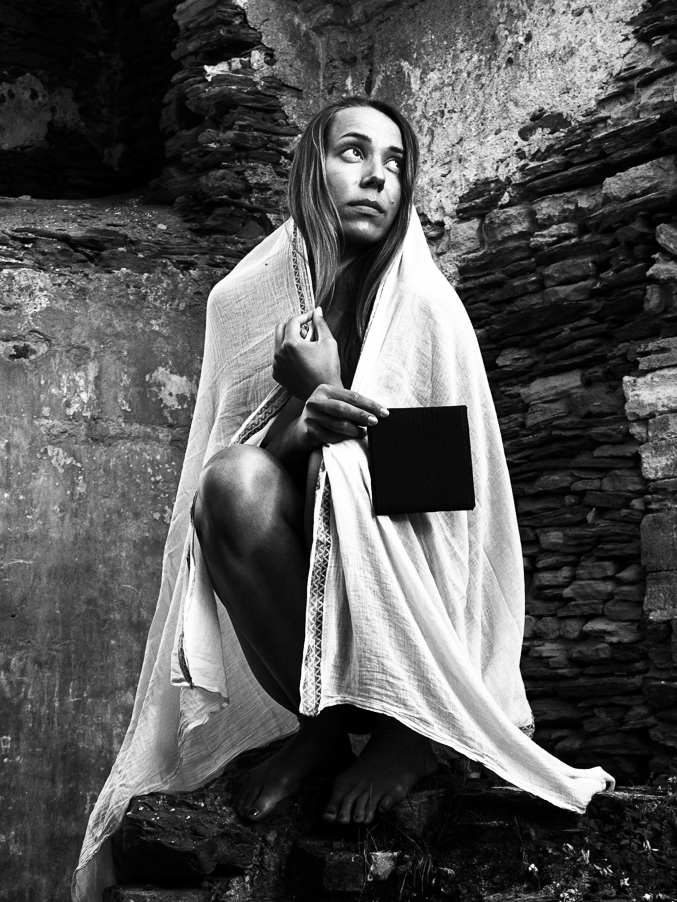
\includegraphics[width=\paperwidth,height=\paperheight,keepaspectratio]{assets/selection/photo-003-cw.png}};
  \fill[white] ([xshift=10mm,yshift=-10mm]current page.north west) rectangle ++(48mm,-16mm);
  \node[anchor=north west,align=left,text width=42mm] at ([xshift=13mm,yshift=-13mm]current page.north west)
    {\metafont\fontsize{6.5}{8}\selectfont 04 / FULL PLATE\\ROTATED 90 CW};
  \node[anchor=south east] at ([xshift=-10mm,yshift=10mm]current page.south east)
    {\metafont\fontsize{6.5}{8}\selectfont IMAGE / SURFACE / POSITION};
\end{tikzpicture}
\newpage

% 19 EXTRA IMAGE / ITS OWN PAGE
\thispagestyle{empty}
\null
\begin{tikzpicture}[remember picture,overlay]
  \node[anchor=center,inner sep=0] at (current page.center)
    {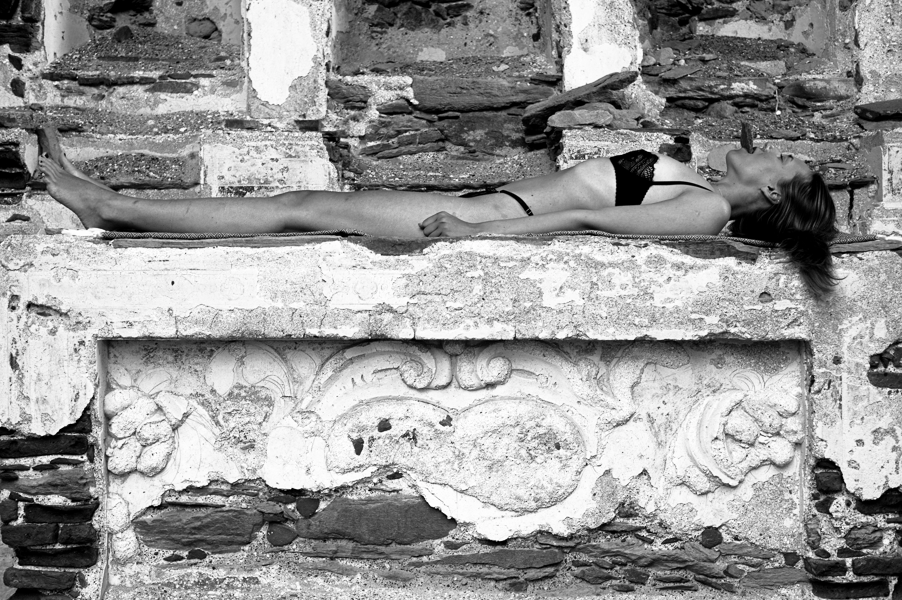
\includegraphics[width=\paperwidth]{assets/selection/photo-005.png}};
  \fill[white,opacity=.92] ([xshift=10mm,yshift=-10mm]current page.north west) rectangle ++(48mm,-17mm);
  \node[anchor=north west,align=left,text width=43mm] at ([xshift=13mm,yshift=-13mm]current page.north west)
    {\metafont\fontsize{6.5}{8}\selectfont EXTRA IMAGE /\\NOT IN CURRENT SELECTION};
  \node[anchor=south east] at ([xshift=-10mm,yshift=10mm]current page.south east)
    {\metafont\fontsize{6.5}{8}\selectfont IMAGE / EXTRA / OPEN POSITION};
\end{tikzpicture}
\newpage

% 20 BACK COVER / CREDITS
\thispagestyle{empty}
\vspace*{45mm}\hspace*{14mm}
\begin{minipage}{179mm}
  \begin{minipage}[t]{112mm}
    {\RaggedRight\displayfont\fontsize{25}{25}\selectfont
      WE ARE COLLECTIVELY RESPONSIBLE\\FOR OUR PRODUCTION.}\par
    \vspace{5mm}
    {\RaggedRight\displayfont\fontsize{19}{21}\selectfont PLAY YOUR POSITION.}\par
    \vspace{8mm}
    {\metafont\fontsize{6.5}{8}\selectfont
      CREDITS / Andr\'es A. Le\'on Baldelli / kumiori III / Ave Palm /\\
      Mai-Brit T\"anava / Kenn-Eerik Kannike.\\[2mm]
      The precise installation responds to the physical dimensions and conditions of the Community Gallery. The sketch describes a system of relations, not a fixed hanging plan.}
  \end{minipage}\hfill
  \begin{minipage}[t]{53mm}
    \centering
    \href{https://takeover-fotografiska.streamlit.app/?a=application}{%
      
\includegraphics[width=48mm]{assets/qr_application.png}}\par
    \vspace{2mm}
    \smallcapsline{ENTER / APPLICATION}\par
    {\metafont\fontsize{5.8}{7}\selectfont
      takeover-fotografiska.streamlit.app\\?a=application}
  \end{minipage}
\end{minipage}
\newpage

% 21 SUGGESTED LISTENING / FINE PRINT
\thispagestyle{empty}
\vspace*{10mm}\hspace*{10mm}
\begin{minipage}{190mm}
  \hrule height .7pt
  \vspace{2.5mm}
  {\metafont\fontsize{7}{8}\selectfont SUGGESTED LISTENING / TERMS AND CONDITIONS OF ATTENTION / STATUS: OPEN}\par
  \vspace{1.5mm}
  \hrule height .3pt
  \vspace{3mm}
  {\fontsize{5.6}{6.35}\selectfont\justifying
  \setlength{\columnsep}{5mm}
  \setlength{\columnseprule}{.25pt}
  \begin{multicols}{3}
  \textbf{PLEASE READ THIS LISTENING INFORMATION CAREFULLY.} An initial listening field around TAKE OVER. Not a soundtrack and not a closed playlist. Records may enter, leave, or acquire new relations as the process develops. By continuing, the listener acknowledges that sequence does not imply hierarchy, that identification may remain provisional, and that relations are active rather than exhaustive. \textbf{01 / JOHANN SEBASTIAN BACH.} Helmut Walcha, \emph{Toccaten und Fugen / Toccatas and Fugues}, LP, Archiv Produktion; Frans-Caspar-Schnitger-Orgel, St. Laurenskerk, Alkmaar; relations: church, organ, architecture, fugue, recurrence; status: identified. Church as resonant architecture; contrapuntal voices separating, returning and remaining autonomous while producing a whole. \textbf{02 / CLASSICAL RITUAL COMPILATION.} \emph{Carmina Burana / Chevauch\'ee des Walkyries / Gnossiennes}; visible works: \emph{Carmina Burana (O Fortuna)}, Erik Satie's \emph{4\`eme Gnossienne} and \emph{5\`eme Gnossienne}; EMI, LP; relations: ritual, fate, repetition, suspension; status: partially identified. A useful collision: monumentality and ritual against Satie's sparse, suspended time. \textbf{03 / AFRICAN HEAD CHARGE.} \emph{Churchical Chant of the Iyabinghi}, LP; relations: chant, assembly, ritual, dub, ecclesia, collective voice; status: identified. Particularly close to the ecclesia thread: assembly enacted through rhythm, chant and collective vocal presence rather than architecture. \textbf{04 / SEPULTURA.} \emph{Arise}, LP; relations: extinction, emergence, violence, rupture, arise; status: identified. Almost absurdly direct in relation to EXTINCTION IN PROGRESS: destruction paired with the imperative to arise. \textbf{05 / PUBLIC SERVICE BROADCASTING.} \emph{The War Room}, record; relations: archive, broadcast, signal, ruins, public voice; status: identified. Archive becomes transmission. Existing recorded material is reactivated and made to speak in another temporal context. \textbf{06 / PROVISIONAL IDENTIFICATION.} Visible title: \emph{AT REAL IRREALE... / ... REALT\`A}; visible artist: KINA; LP; relations: real, unreal, mediation, image, signal; status: needs identification. Keep provisional until the exact artist, title, and edition are checked. The visible real/irreale language is already relevant to the portal logic. \textbf{07 / RAGE AGAINST THE MACHINE.} \emph{Rage Against the Machine}, LP; relations: resistance, body, institution, combustion, political action; status: identified. Body as irreversible political signal. An image that cannot be separated comfortably from the act it records. \textbf{08 / WOLFGANG AMADEUS MOZART.} Berliner Philharmoniker, Herbert von Karajan, \emph{Eine kleine Nachtmusik / Divertimento KV 287}, Deutsche Grammophon, LP; relations: night, divertimento, gathering, social music; status: identified. Night as social space rather than darkness alone. Music written to occupy an occasion. \textbf{09 / FABRIZIO DE ANDR\'E.} \emph{Non al denaro non all'amore n\'e al cielo}; visible track: \emph{Un blasfemo}; LP; relations: cemetery, dead speaking, biography, community, memory; status: identified. Extremely close to the photographic narrative: a community reconstructed through voices of the dead. The cemetery speaks person by person. \textbf{10 / COLLAGE.} \emph{K\"aokiri}, LP; relations: Estonia, polyphony, folk memory, collective voice, Tallinn; status: identified. A local and polyphonic anchor: inherited song reorganised through a collective vocal language. \textbf{11 / DJ METATRON.} \emph{2 The Sky}, Giegling, catalogue Giegling 18, 2016, record; cover: white sleeve with two hand-drawn blue crosses; relations: sky, ascent, electronic music, signal; status: identified. The white sleeve with the two hand-drawn blue crosses; the cover match is confirmed. \textbf{12 / GLASS BEAMS.} \emph{Mahal}, Ninja Tune, 2024, EP; copper/gold sleeve; visible tracks: \emph{Horizon}, \emph{Mahal}, \emph{Orb}, \emph{Snake Oil}, \emph{Black Sand}; relations: horizon, ritual, psychedelic music, mediation; status: identified. The copper/gold record at upper right. A five-track EP moving through horizon, orbit, ritual and mirage-like repetition. \textbf{GENERAL PROVISIONS.} Listening may occur in whole or in part, in order or out of order, alone or in assembly, before, during, or after the exhibition. No entry shall be construed as a mandatory soundtrack, definitive interpretation, fixed programme, endorsement of closure, or waiver of the listener's right to introduce another relation. The field remains open.
  \end{multicols}}
  \vfill
  \hrule height .3pt
  \vspace{2mm}
  {\metafont\fontsize{5.5}{6.5}\selectfont TAKE OVER / LISTENING ADDENDUM / SOURCE: TAKEOVER-LISTENING V1 / SUBJECT TO CHANGE WITHOUT NOTICE}
\end{minipage}
\end{document}
